\chapter{Analysis of Results}
We are going to analyze the resulting models after training them as specified in Chapter~\ref{methods:training}.

As the first part, we are going to analyze how the training went and take a look at the results of the metric-based evaluation (see Chapter~\ref{methods:evaluation}). Because we identified some problems with this quantitative analysis, we then show that progress was indeed achieved throughout the training and go into detail why the results of the evaluation are as bad as they are. This includes an analysis into the language model to determine why the models often time respond with generic outputs.

The next part is then dedicated to comparing our models with the results from the paper of Vinyals and Le~\cite{Vinyals:2015} and with the CleverBot chatbot.

The subjects of the last part are analysis related beam-search and the soft-attention mechanism.\todo{Evtl. diesen umschreiben/ergänzen}

\section{How Did The Training Go?}
First, let us start by analyzing the evolution of the models with regard to the available performance metrics throughout the time period of the training. Below, in Figures~\ref{results:learning_process:metrics:opensubtitles} and~\ref{results:learning_process:metrics:reddit}, one can see the development of the cross-entropy loss and perplexity values on the training datasets for the two different models.

\paragraph{OpenSubtitles} What is eye-catching when comparing the two is that the OpenSubtitles seems to have much more variance in its performance on the validation set then the Reddit model. This is most probably caused by the fact that the OpenSubtitles dataset is much more noisey than the Reddit, as also noticed by others\cite{Vinyals:2015}. This has to do with the missing information about turn taking, which means it is certainly possible that consecutive utterances in the dataset may be uttered by the same person even though we treat it if it was uttered by two different persons. Also, there is the problematic with the time lags between utterances as analyzed in Chapter~\ref{data:opensubtitles:time_lag_analysis}. In contrast, with the Reddit dataset we always know who uttered a comment and hence can build a dataset which ensures that the dialogs make sense from a structural perspective.

\begin{figure}[H]
	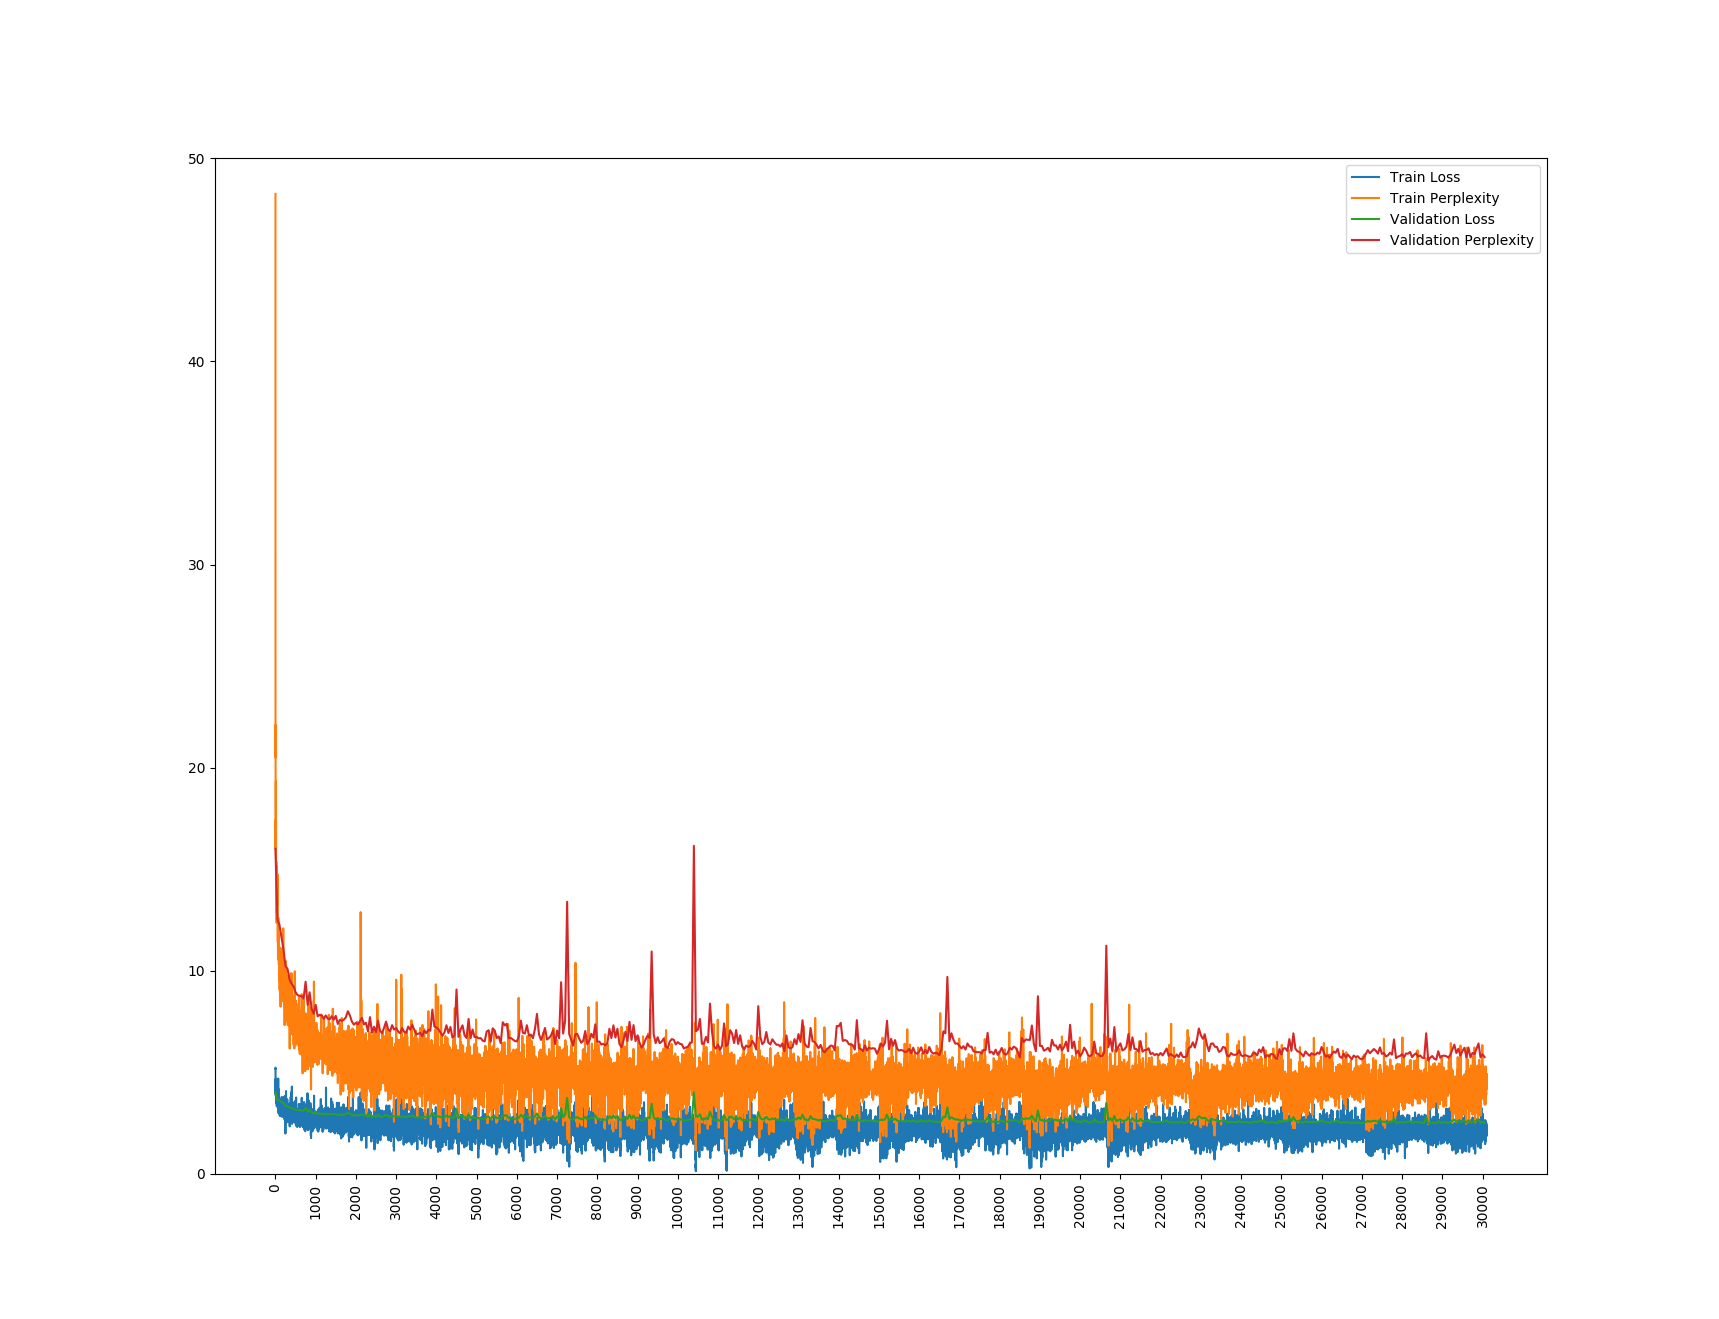
\includegraphics[width=\linewidth]{img/plots/opensubtitles_not_reversed/train_metrics.png}
	\caption{Development of the loss and perplexity on the training and validation set throughout the training of the OpenSubtitles model. One tick on the x-axis is equal to $100$ batches processed.}
	\label{results:learning_process:metrics:opensubtitles}
\end{figure}

\paragraph{Reddit} The learning process of the Reddit model looks find, but it also has a peculiarity, namely the dips in the training loss and perplexity. These dips occur about every $300,000$ to $400,000$ batches. They are also present in the development of the validation loss and perplexity, but are not as apparent as in the training metrics. We cannot explain this behaviour currently. We assume that this comes from the fact...\todo{Maybe we should be able?!} The variance however is much smaller than with the OpenSubtitles model, which strengthens our argument, that a well-structured dataset helps a lot when training such systems as it confuses the model much less.\todo{maybe rewrite this sentence somehow}

\begin{figure}[H]
	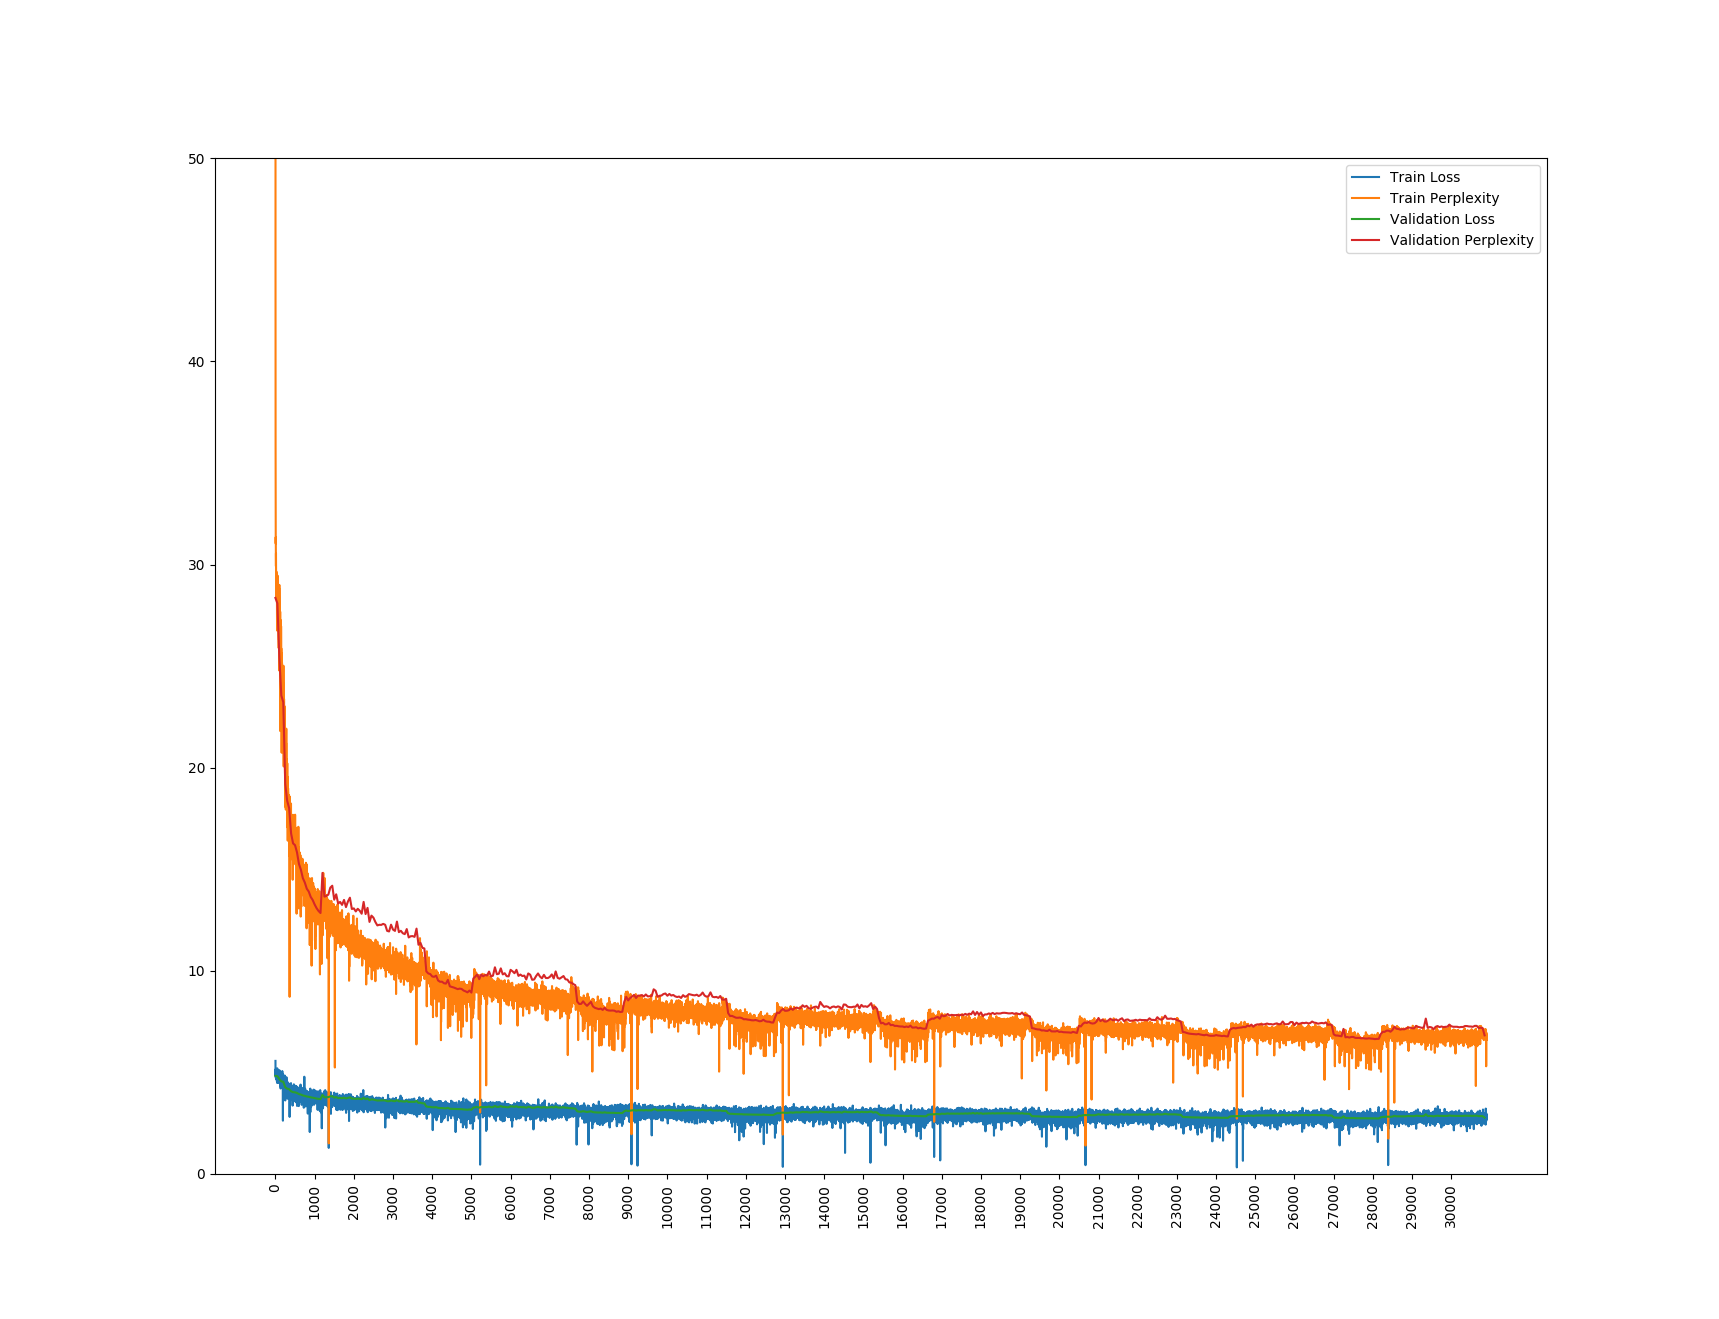
\includegraphics[width=\linewidth]{img/plots/reddit/train_metrics.png}
	\caption{Development of the loss and perplexity on the training and validation set throughout the training of the Reddit model. One tick on the x-axis is equal to $100$ batches processed.}
	\label{results:learning_process:metrics:reddit}
\end{figure} 

\paragraph{The Training Seems Successful} From the looks of the plots, it looks like the training went fine for both models, as both of them have degrading loss and perplexity. We also saw differences in how the models have evolved over the time span of the training, especially the dips in the Reddit model, but we cannot conclude anything from this right now. After we have analyzed the training process, we are now focusing on the performance of the models on the test datasets.

\section{Performance on Test Datasets}
After we have seen that the training process looks fine, we are going to asses the performance of these models on our test datasets. Here we use the same metrics as within the training, namely the cross-entropy loss and perplexity values. We have evaluated each model on the respective test dataset for each checkpoint we have created while training (see Chapter~\ref{methods:training}).

\paragraph{Surprising Results} The results on the test set are quite the opposite of the results from the training process (see Figures~\ref{result:test_performance:opensubtitles} and~\ref{result:test_performance:reddit}), where both of the models are getting worse over time. We did not expect that, but nevertheless, we are going to analyze the problem.\todo{Maybe some more clarification on what analyse means?} The results of the OpenSubtitles model seem to vary across the different checkpoints, with the best result having a perplexity of $71.07$ and a loss of $6.15$ and coming from the evaluation with the first checkpoint.\todo{Values for reddit model in text} The best result of the Reddit model is also achieved on the first checkpoint, with all other checkpoints having a worse perplexity.

This result stands in contradiction to what we have expected. Instead of the loss values going up, we would have expected it to go down in the same way as it did on the training and validation datasets. We assume, that this has to do with the cross-entropy loss and hence the perplexity being not the best fit metrics to evaluate such models, especially in a conversational context where the variety of correct answers can be immensely high. For this reason, we proposed a third performance metric, namely the usage of Sent2Vec~\cite{Pgj:2017} embeddings, to measure the similarity between the expected and generated responses. Before we are going to do this analysis, we want to take a look at different samples from both models to show that they indeed improved over time, even thought the test metrics tell a different story.

\begin{figure}[H]
	\minipage{0.5\textwidth}
	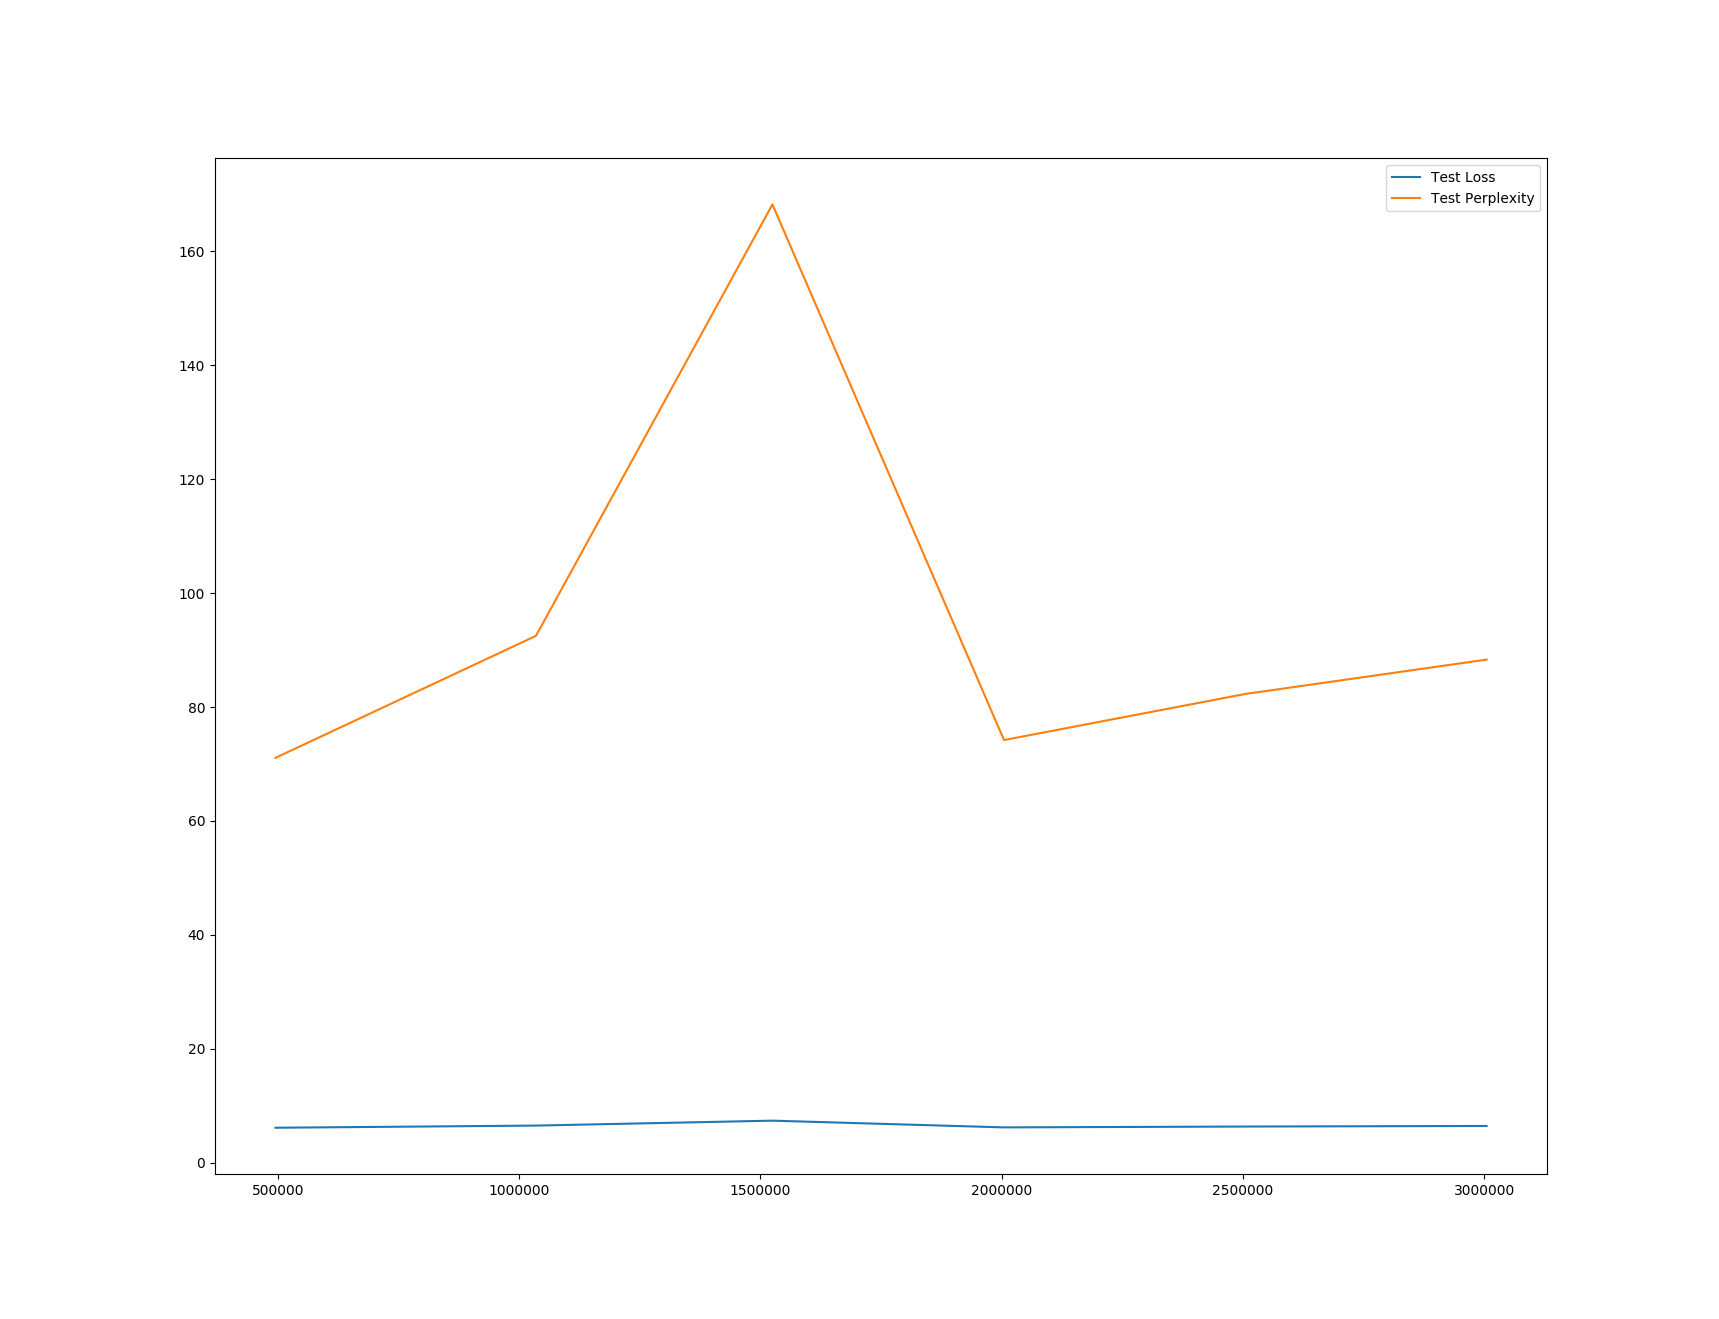
\includegraphics[width=\linewidth]{img/plots/opensubtitles_not_reversed/test_metrics_both.png}
	\centering
	\small
	\text{The loss and perplexity.}
	\endminipage\hfill
	\minipage{0.5\textwidth}
	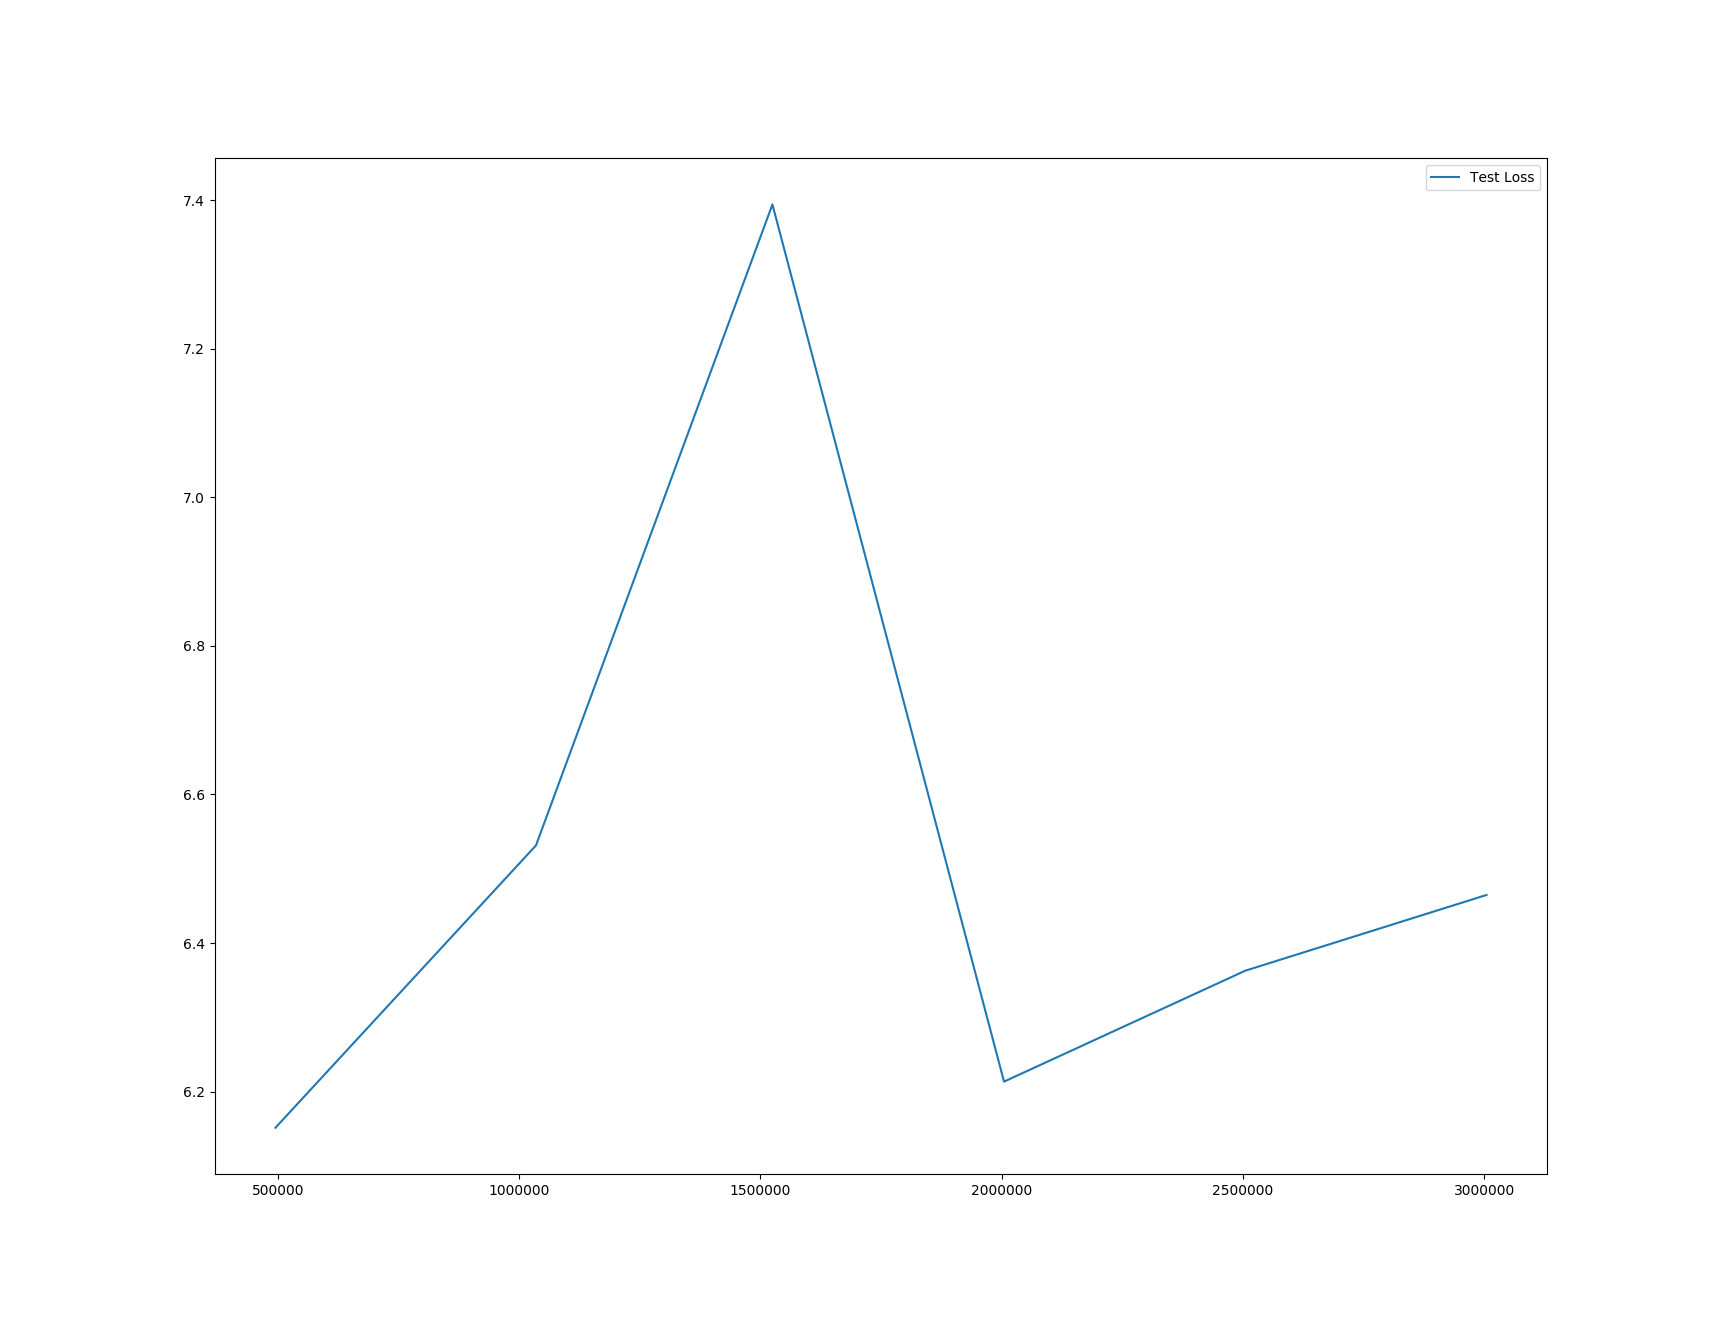
\includegraphics[width=\linewidth]{img/plots/opensubtitles_not_reversed/test_metrics_loss.png}
	\centering
	\small
	\text{Only the loss.}
	\endminipage\hfill
	\caption{The loss and perplexity by running the six different snapshots against the test dataset using the OpenSubtitles model.}
	\label{result:test_performance:opensubtitles}
\end{figure}

\begin{figure}[H]
	\minipage{0.5\textwidth}
	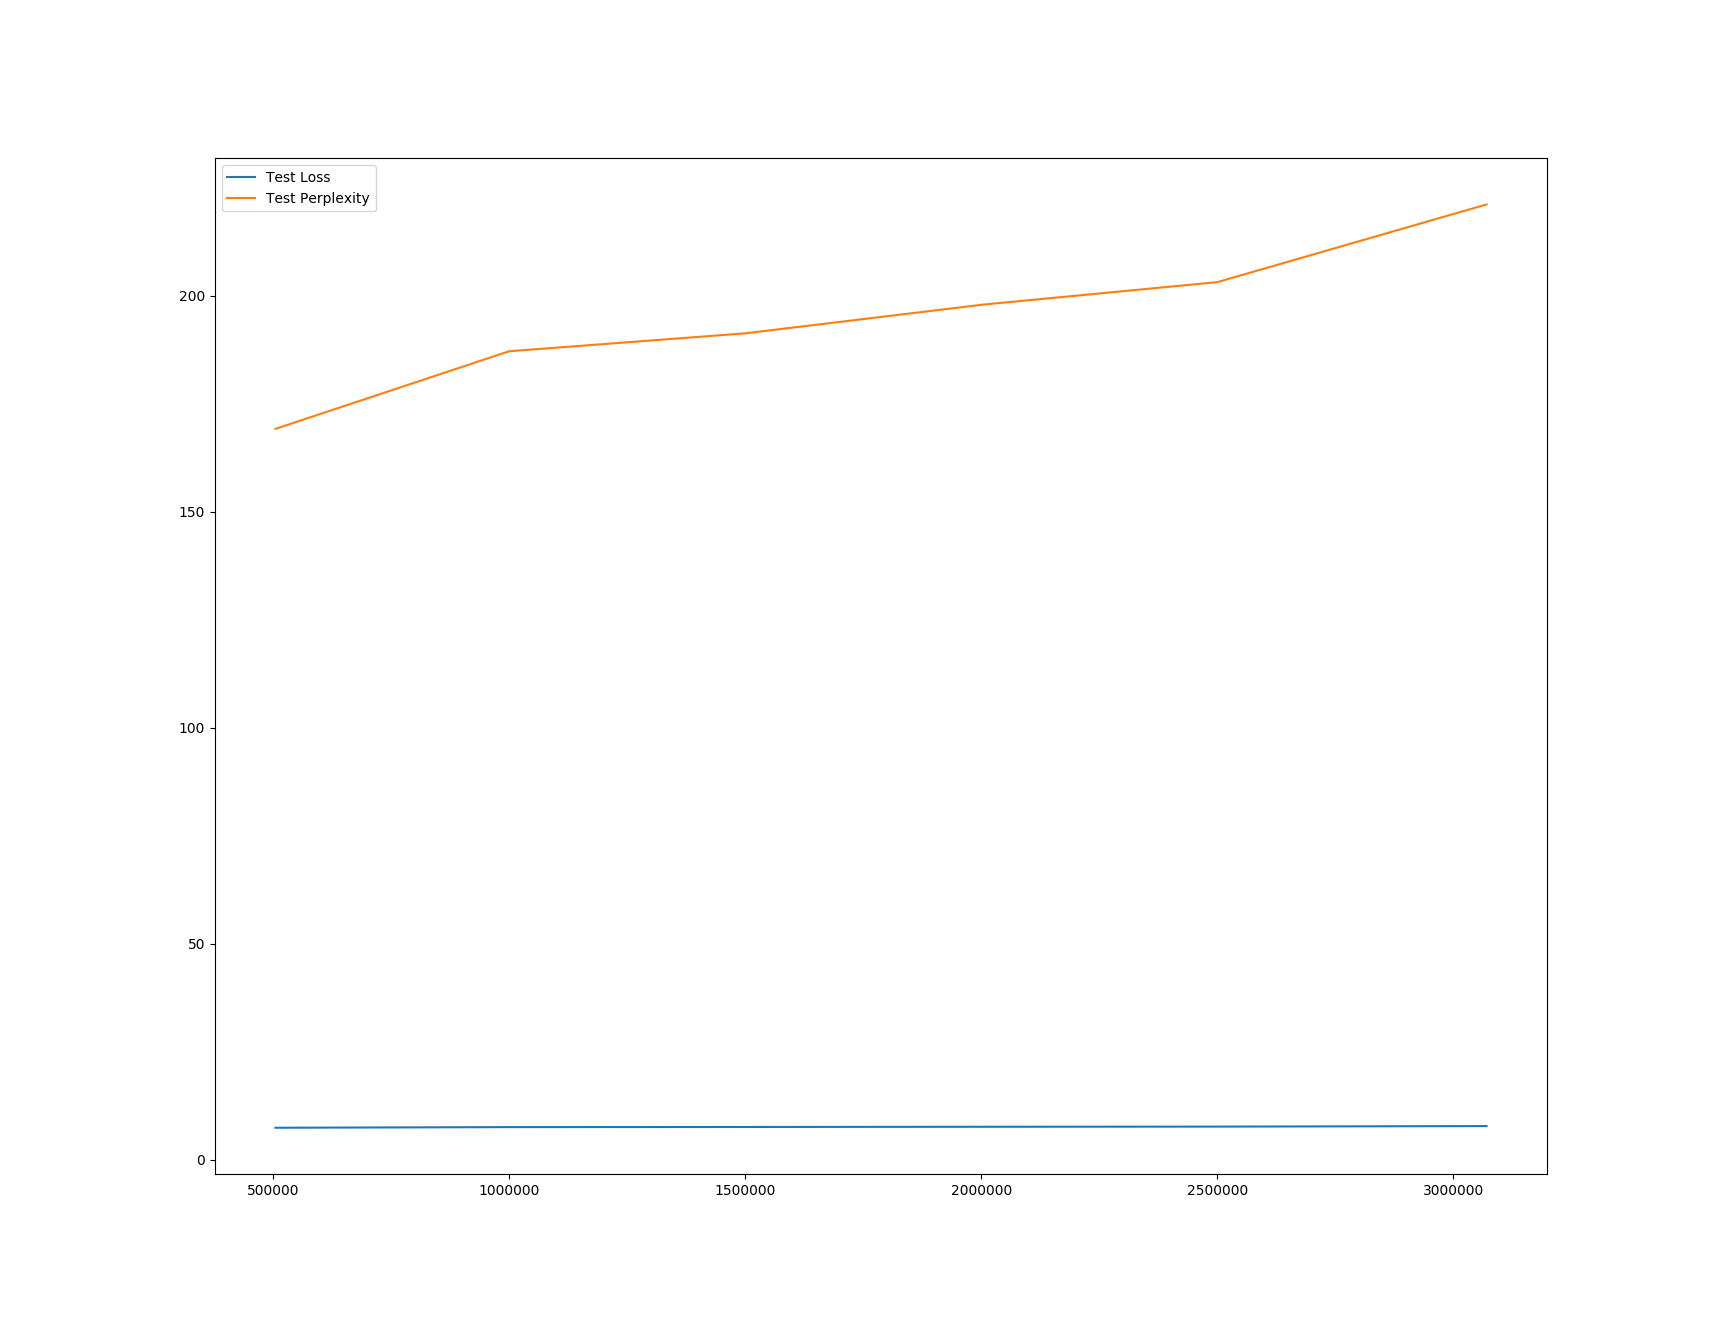
\includegraphics[width=\linewidth]{img/plots/reddit/test_metrics_both.png}
	\centering
	\small
	\text{The loss and perplexity.}
	\endminipage\hfill
	\minipage{0.5\textwidth}
	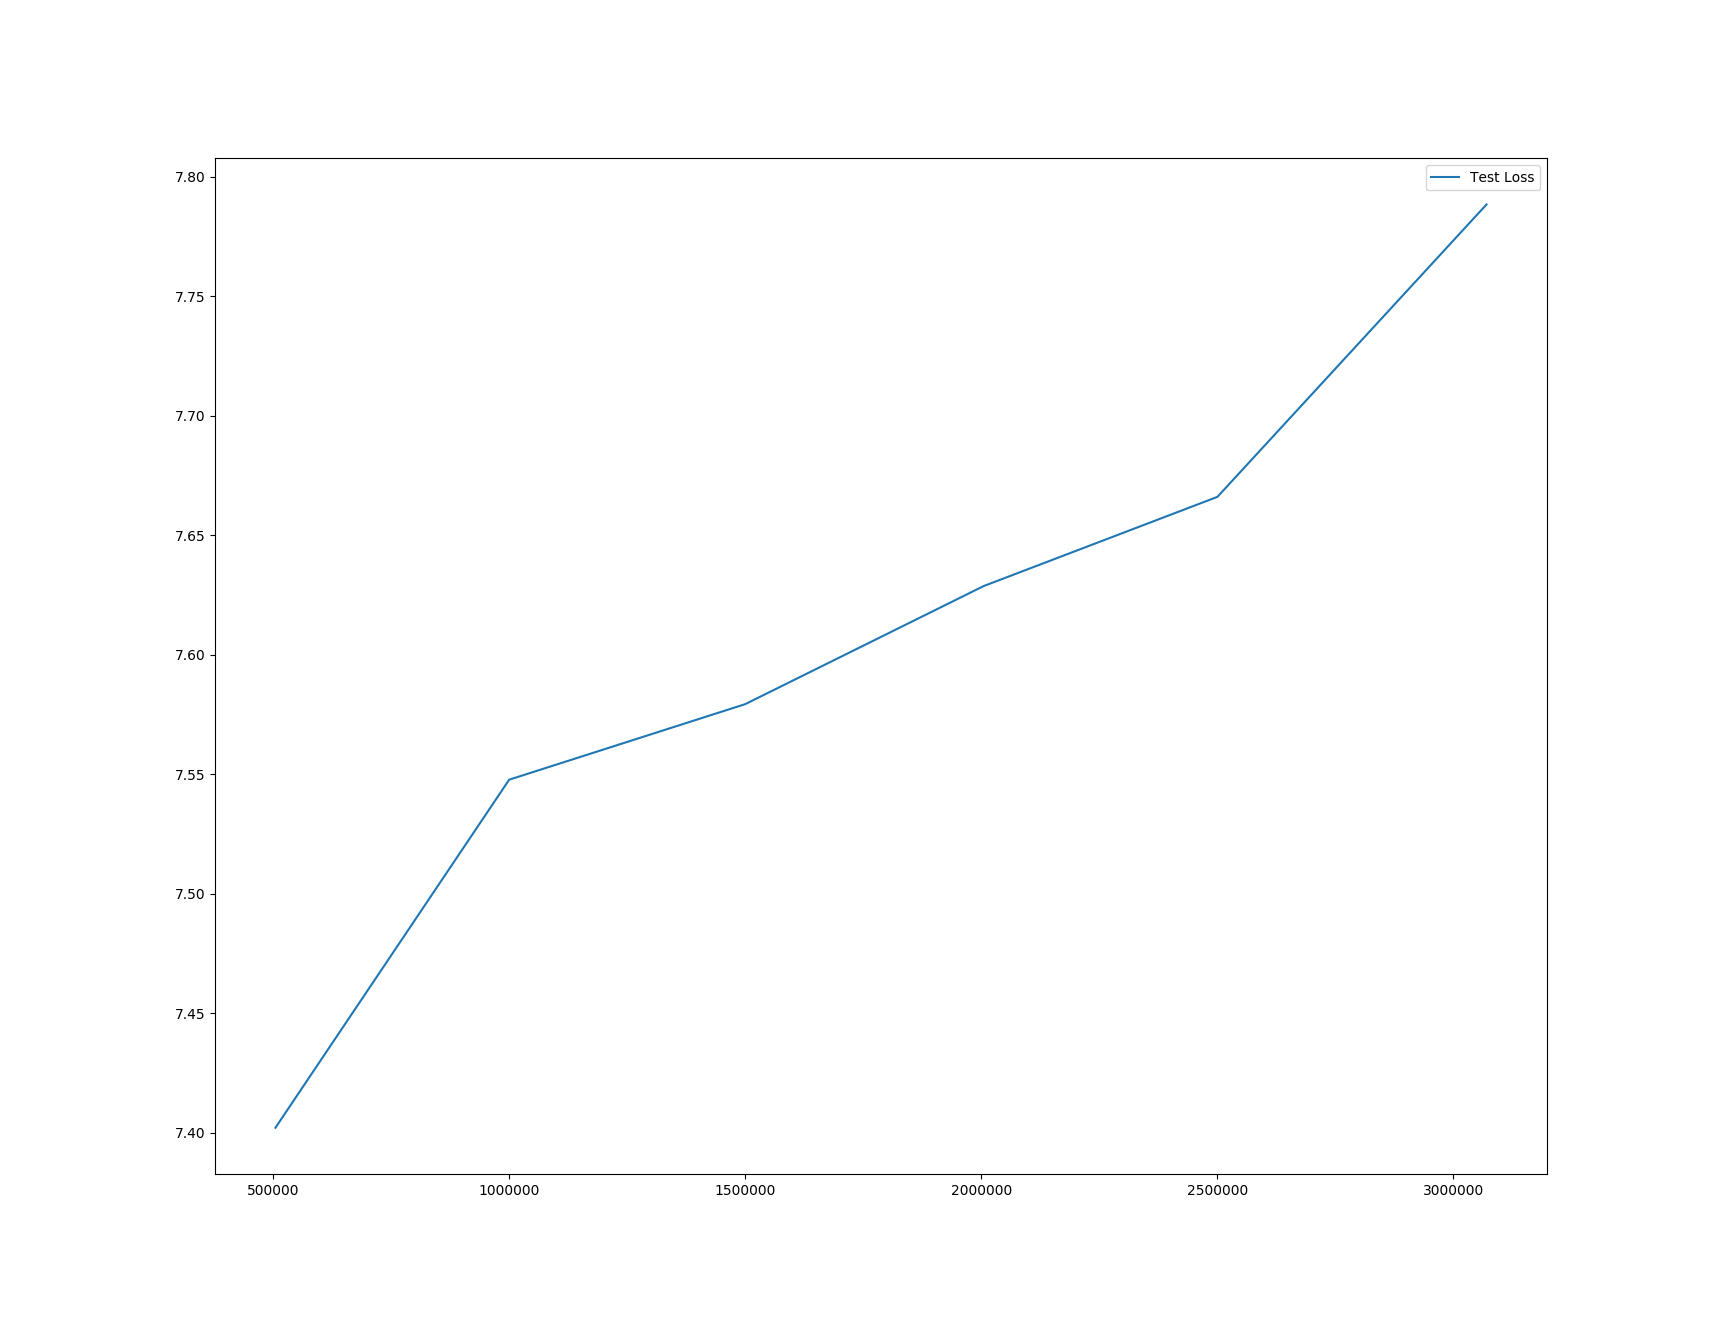
\includegraphics[width=\linewidth]{img/plots/reddit/test_metrics_loss.png}
	\centering
	\small
	\text{Only the loss.}
	\endminipage\hfill
	\caption{The loss and perplexity by running the six different snapshots against the test dataset using the Reddit model.}
	\label{result:test_performance:reddit}
\end{figure}

\paragraph{Is Progress Achieved?} As the results of evaluating the models on the test dataset has shown, it seems that the models did not make an meaningful progress throughout the training. Even worse, it looks like the models have become worse over time. For this reason, we decided that we would like to evaluate the model by hand and see if the generated responses improve when using the different six snapshots of the models. We opted for four different input sentences, that means two for each model, and generated responses for each of the snapshots. The results can be seen in the Table~\ref{results:example_output:reddit} for the Reddit model and Table~\ref{results:example_output:opensubtitles} for the OpenSubtitles model.

\begin{table}[H]
	\centering
	\ra{1.3}
	\begin{adjustbox}{max width=\textwidth}
		\begin{tabular}{ll}
			\toprule
			Input: 	& \texttt{Do you like Joffrey from game of thrones?}\\
			\midrule
			0.5M: 	& \texttt{i m not sure if you re a fan of the movie ,}\\
			& \texttt{but i m not sure if you re a fan of the movie .}\\
			1.0M: 	& \texttt{i m not a fan of the game , but i m not sure if it s a game or not .}\\
			1.5M:	& \texttt{i do nt know what i m talking about .}\\
			2.0M:	& \texttt{i do nt }\\
			2.5M:	& \texttt{i do nt know what i m talking about .}\\
			3.0M:	& \texttt{i do nt know , i just do nt like him .}\\
			\midrule
			Input: 	& \texttt{Which movie can you recommend me?}\\
			\midrule
			0.5M: 	& \texttt{the}\\
			1.0M: 	& \texttt{the movie .}\\
			1.5M:	& \texttt{the one with the}\\
			2.0M:	& \texttt{the dark knight rises}\\
			2.5M:	& \texttt{the prestige}\\
			3.0M:	& \texttt{the movie}\\
			\bottomrule
		\end{tabular}
	\end{adjustbox}
	\caption{Two example dialogs with the Reddit model with one response per snapshot.}
	\label{results:example_output:reddit}
\end{table}
\todo{Format so that all look the same, probably by using tabularx and an X column}

\begin{table}[H]
	\centering
	\ra{1.3}
	\begin{adjustbox}{max width=\textwidth}
		\begin{tabular}{ll}
			\toprule
			Input: 	& \texttt{Are you a man or a woman?}\\
			\midrule
			0.5M: 	& \texttt{no , no , no}\\
			1.0M: 	& \texttt{no}\\
			1.5M:	& \texttt{i m not a man}\\
			2.0M:	& \texttt{i m not a woman}\\
			2.5M:	& \texttt{i m a man}\\
			3.0M:	& \texttt{i m not a woman}\\
			\midrule
			Input: 	& \texttt{Why should it not be a good idea to improve you?}\\
			\midrule
			0.5M: 	& \texttt{no}\\
			1.0M: 	& \texttt{i don t know}\\
			1.5M:	& \texttt{because i love you}\\
			2.0M:	& \texttt{because i m a good man}\\
			2.5M:	& \texttt{i m just trying to make a good decision}\\
			3.0M:	& \texttt{i m not a good idea}\\
			\bottomrule
		\end{tabular}
	\end{adjustbox}
	\caption{Two example dialogs with the OpenSubtitles model with one response per snapshot.}
	\label{results:example_output:opensubtitles}
\end{table}

As seen in the examples above, there has indeed been an improvement in the answers, what stands in contradiction to the development of the performance of the models on the test datasets. Our reasonable suspicion from this is, again, that the cross-entropy loss and perplexity are not fit to asses if the responses are meaningful. As we have already described in Chapter~\ref{fundamentals:sent2vec_test}, we were aware of the fact, that our current set of metrics is not satisfying for evaluating if the responses are meaningful, why we decided to use yet another metric, namely Sent2Vec embeddings, which we are going to use in the next section.

\paragraph{Sent2Vec Analysis} As described in Chapter~\ref{fundamentals:sent2vec_test}, we use Sent2Vec embeddings for measuring the semantic similarity between the generated and expected responses on the test dataset. For this purpose, we have used the pretrained models available on the GitHub page of the project\footnote{https://github.com/epfml/sent2vec}. We have decided, that we use both the \emph{Twitter} and \emph{Wikipedia} models for the assessment. The results can be seen in the Figures~\ref{results:sent2vec:opensubtitles:results} and~\ref{results:sent2vec:reddit:results}. What can be directly seen is that both the Reddit and OpenSubtitles models perform better on the pretrained Wikipedia model in comparison to the pretrained twitter model. This probably has to do with the fact that ``compressed'' language used when writing tweets (e.g. ``w/o'' instead of ``without'') and with the coverage of the vocabulary. In conclusion, the results of this analysis are dependent on the Sent2Vec model, as expected. However, both results are pretty bad, with the Reddit results being much better than the OpenSubtitles, about twice as good (see Tables~\ref{results:sent2vec:opensubtitles:results_table} and~\ref{results:sent2vec:reddit:results_table}). The OpenSubtitles model starts with an average similarity of $0.167$ for the first snapshot and climbs up to $0.204$ for the last snapshot. The Reddit model starts with an average value of $0.336$ for the first snapshot and increases to $0.359$ for the last snapshot. This means, that the responses of the Reddit model match the expected responses much better from a semantic perspective as the responses of the OpenSubtitles model do. In summary, the results of both models are highly pretty bad, as the maximum similarity is $1.0$.

\begin{figure}[H]
	\minipage{0.5\textwidth}
	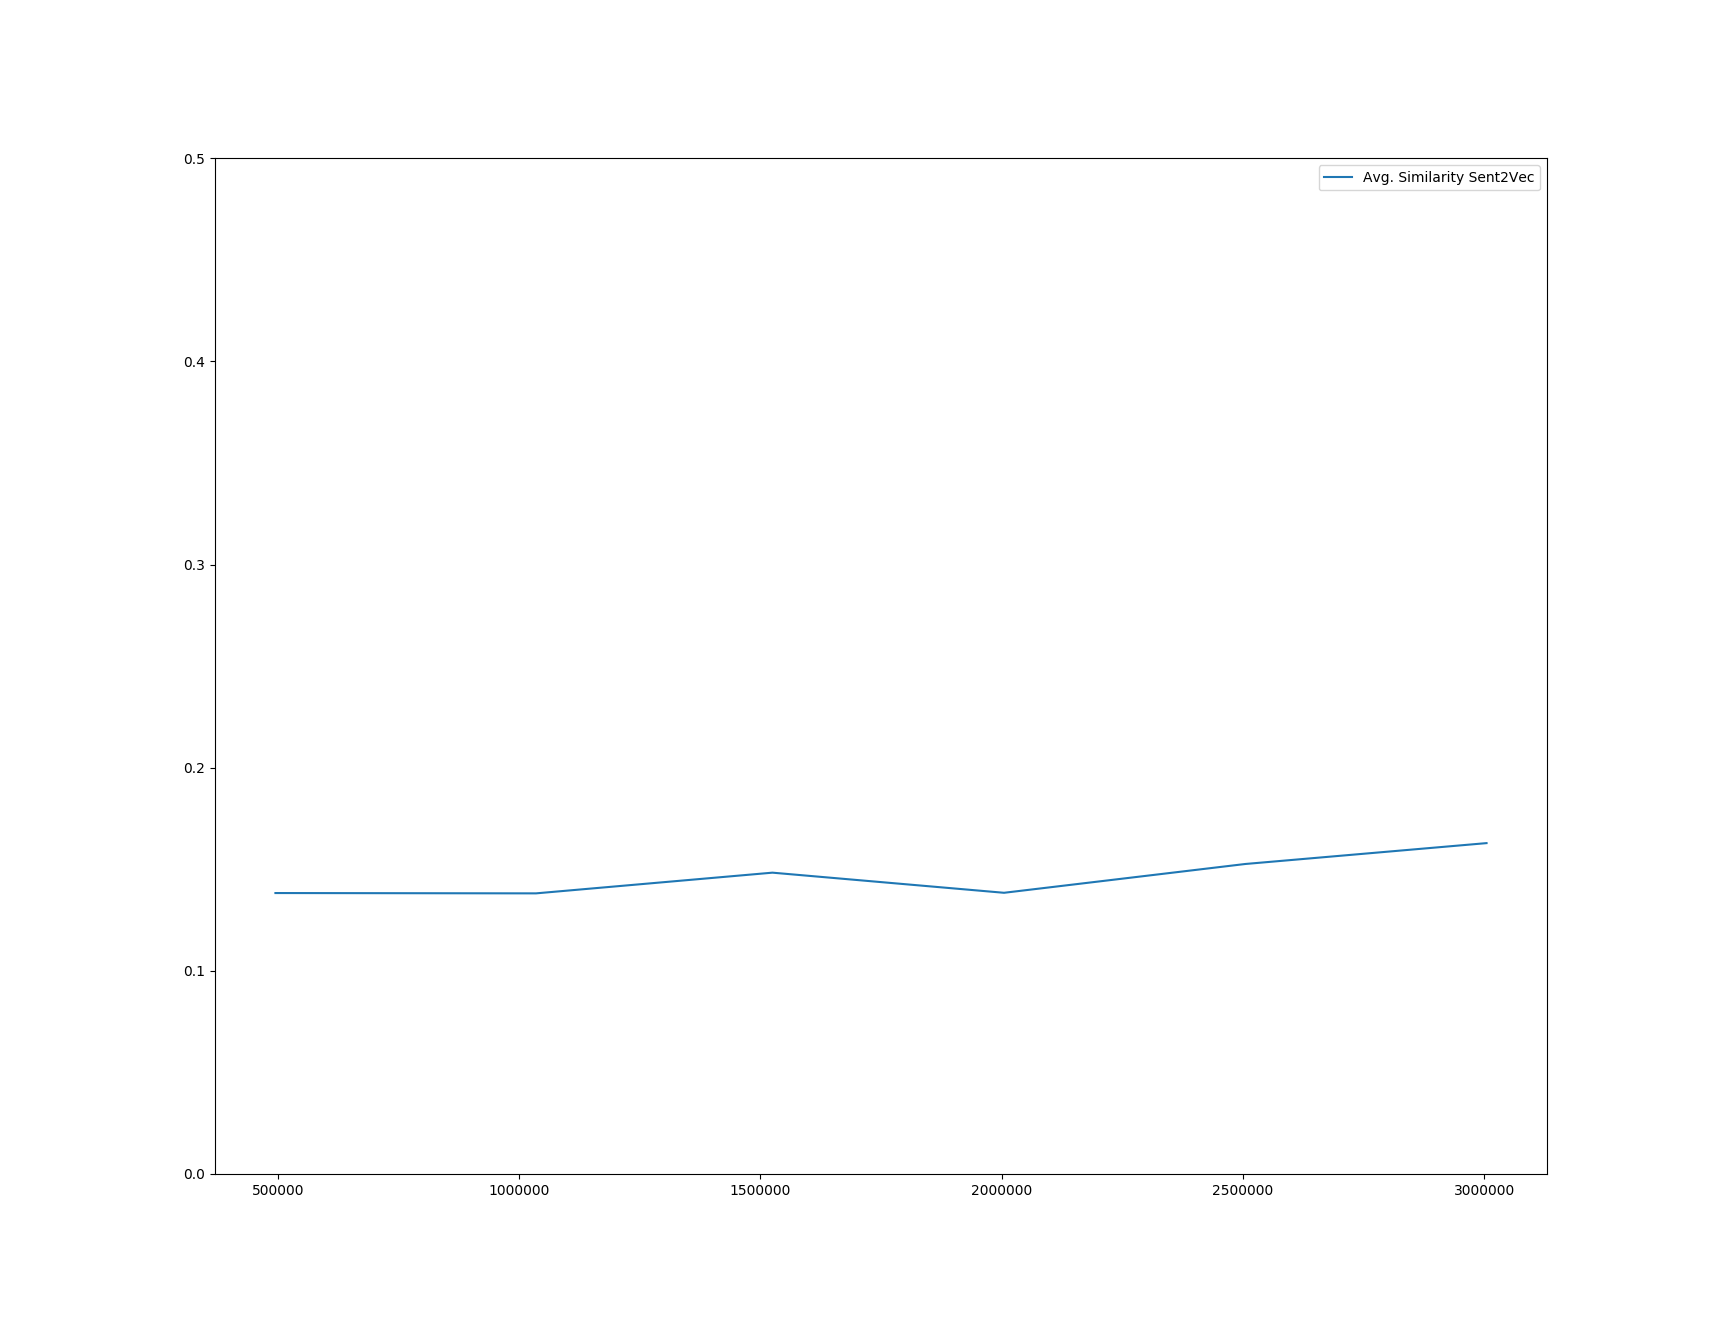
\includegraphics[width=\linewidth]{img/plots/opensubtitles_not_reversed/s2v_wiki_cosine_similarity.png}
	\centering
	\small
	\text{Wikipedia}
	\endminipage\hfill
	\minipage{0.5\textwidth}
	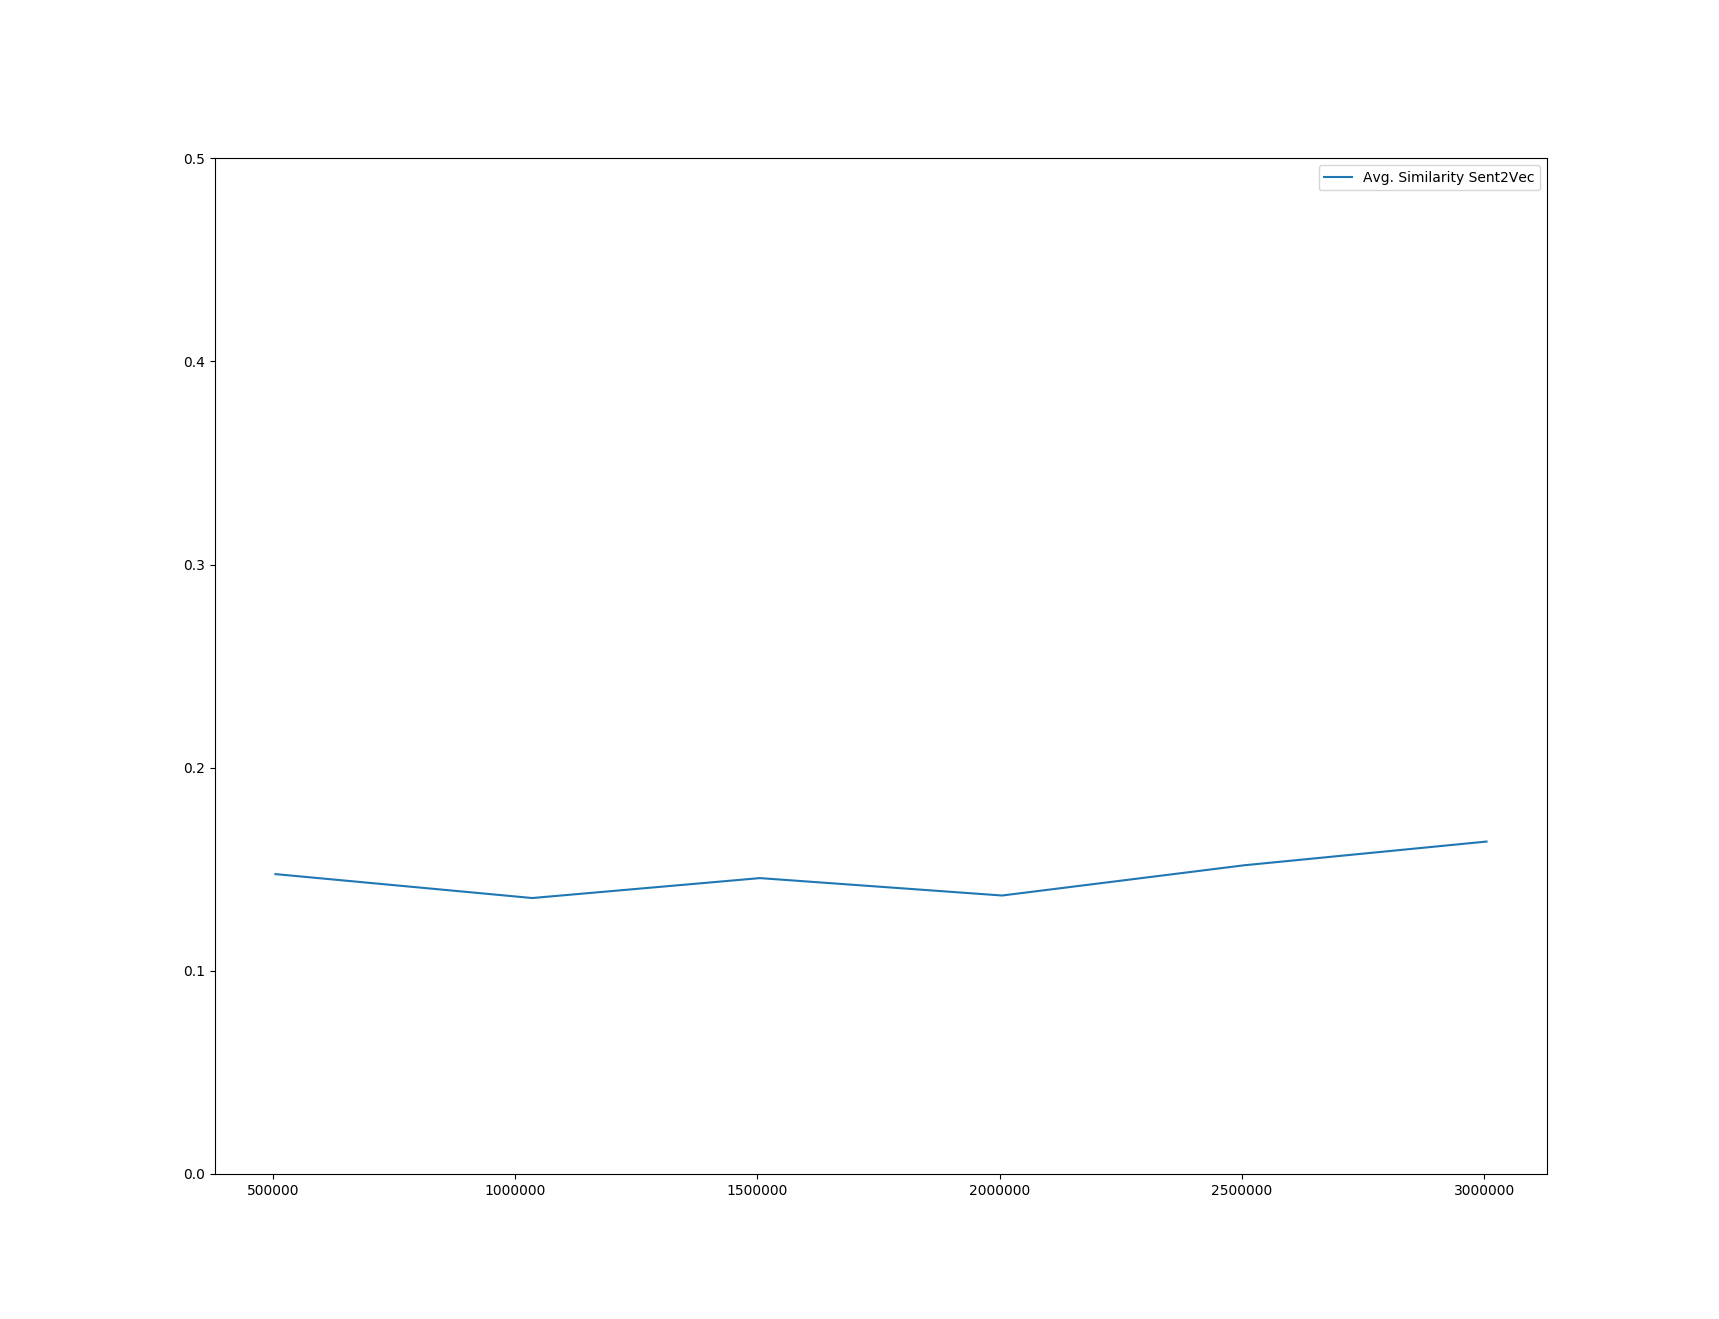
\includegraphics[width=\linewidth]{img/plots/opensubtitles_not_reversed/s2v_twitter_cosine_similarity.png}
	\centering
	\small
	\text{Twitter}
	\endminipage\hfill
	\caption{Results of the evaluation with Sent2Vec on the outputs of the OpenSubtitles models using the pretrained models. The ticks on the x-axis show the different snapshots and the y-axis the average semantic similarity when using Sent2Vec for each snapshot.}
	\label{results:sent2vec:opensubtitles:results}
\end{figure}

\begin{table}[H]
	\centering
	\ra{1.3}
	\begin{adjustbox}{max width=\textwidth}
		\begin{tabular}{lcc}
			\toprule
			Snapshot & Avg. Similarity (Wikipedia) & Avg. Similarity (Twitter)\\
			\midrule
			0.5M & $0.16749$ & $0.13827$\\
			1.0M & $0.19111$ & $0.13811$\\
			1.5M & $0.19418$ & $0.14831$\\
			2.0M & $0.19176$ & $0.13840$\\
			2.5M & $0.20118$ & $0.15258$\\
			3.0M & $0.20452$ & $0.16285$\\
			\bottomrule
		\end{tabular}
	\end{adjustbox}
	\caption{The average similarities when applying the Sent2Vec metric on the expected and generated responses from the OpenSubtitles model.}
	\label{results:sent2vec:opensubtitles:results_table}
\end{table}

\begin{figure}[H]
	\minipage{0.5\textwidth}
	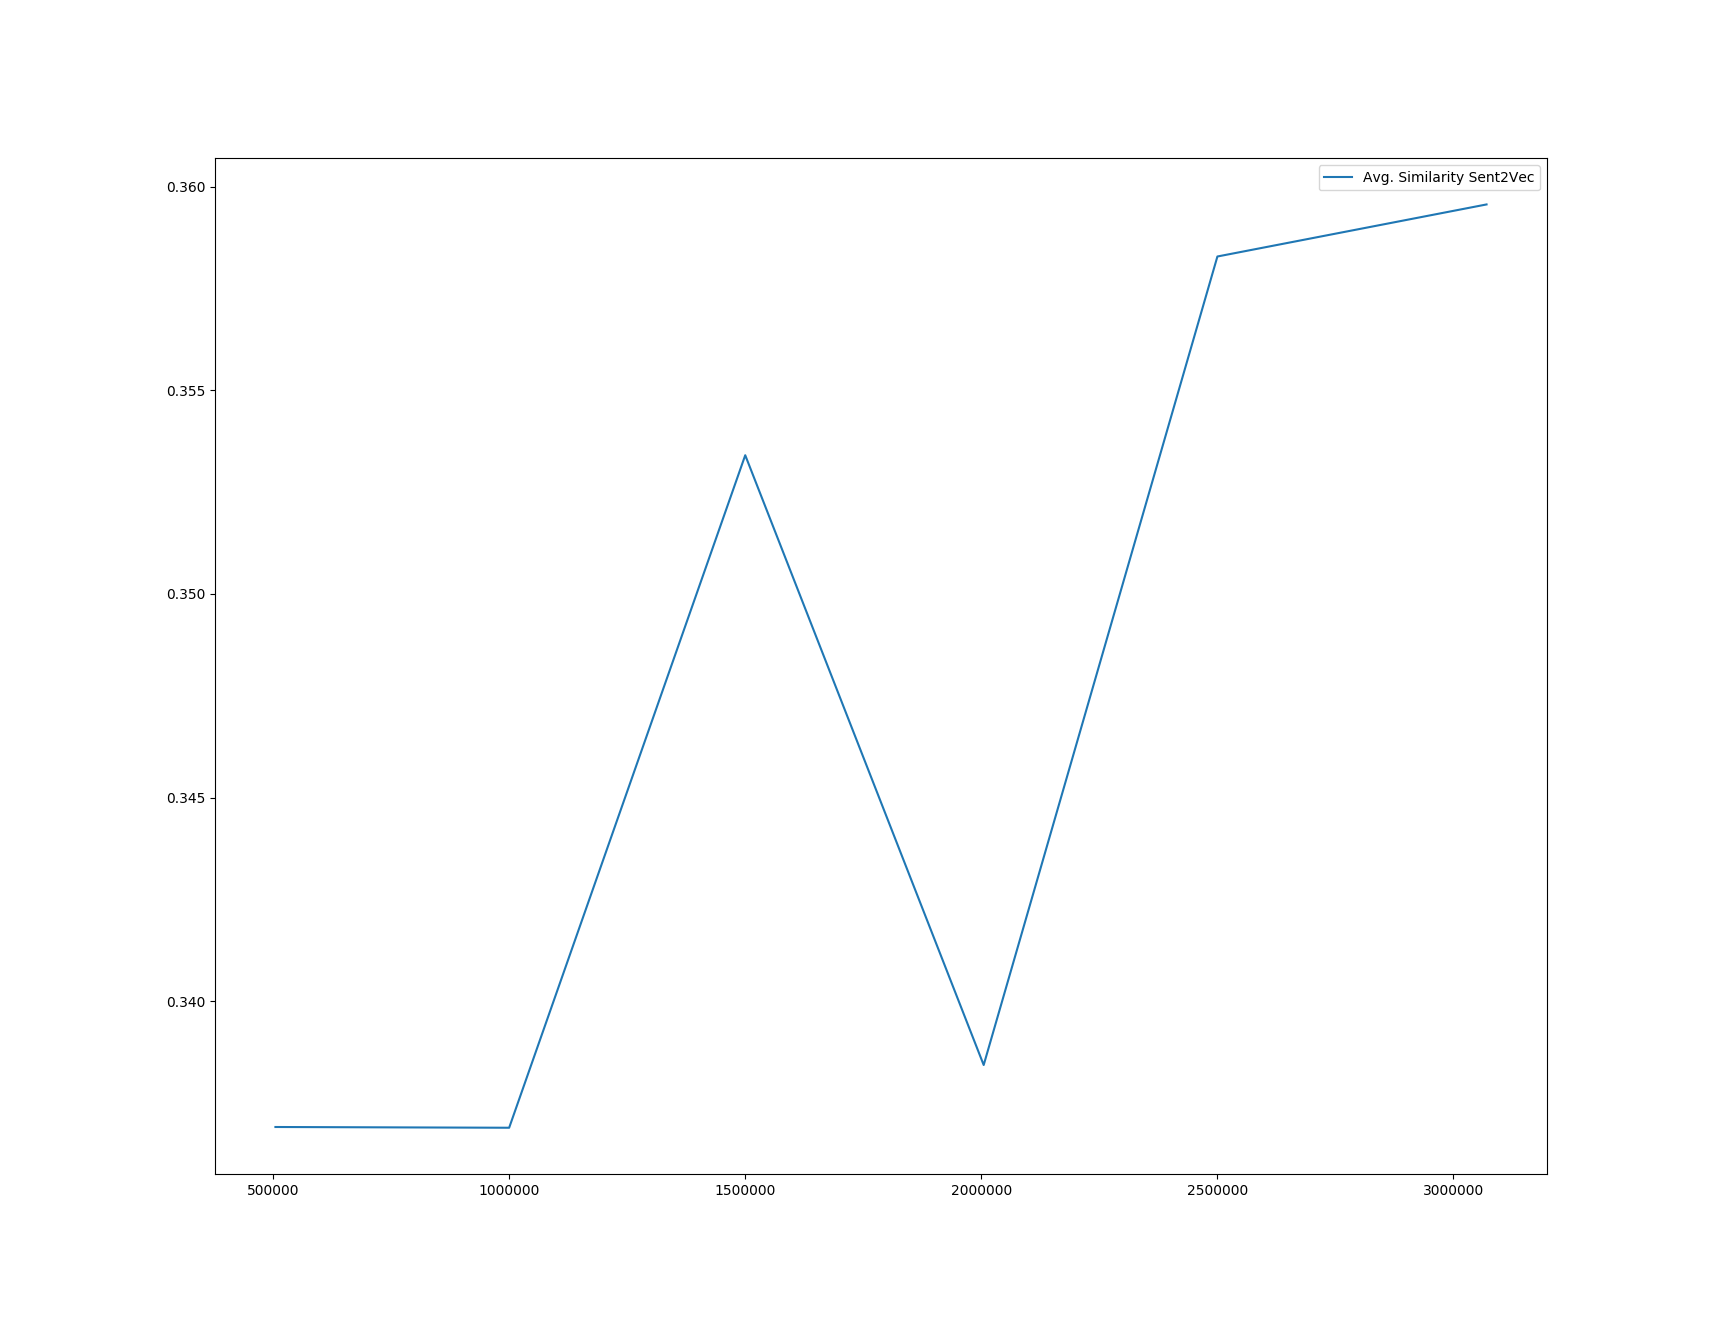
\includegraphics[width=\linewidth]{img/plots/reddit/s2v_wiki_cosine_similarity.png}
	\centering
	\small
	\text{Wikipedia}
	\endminipage\hfill
	\minipage{0.5\textwidth}
	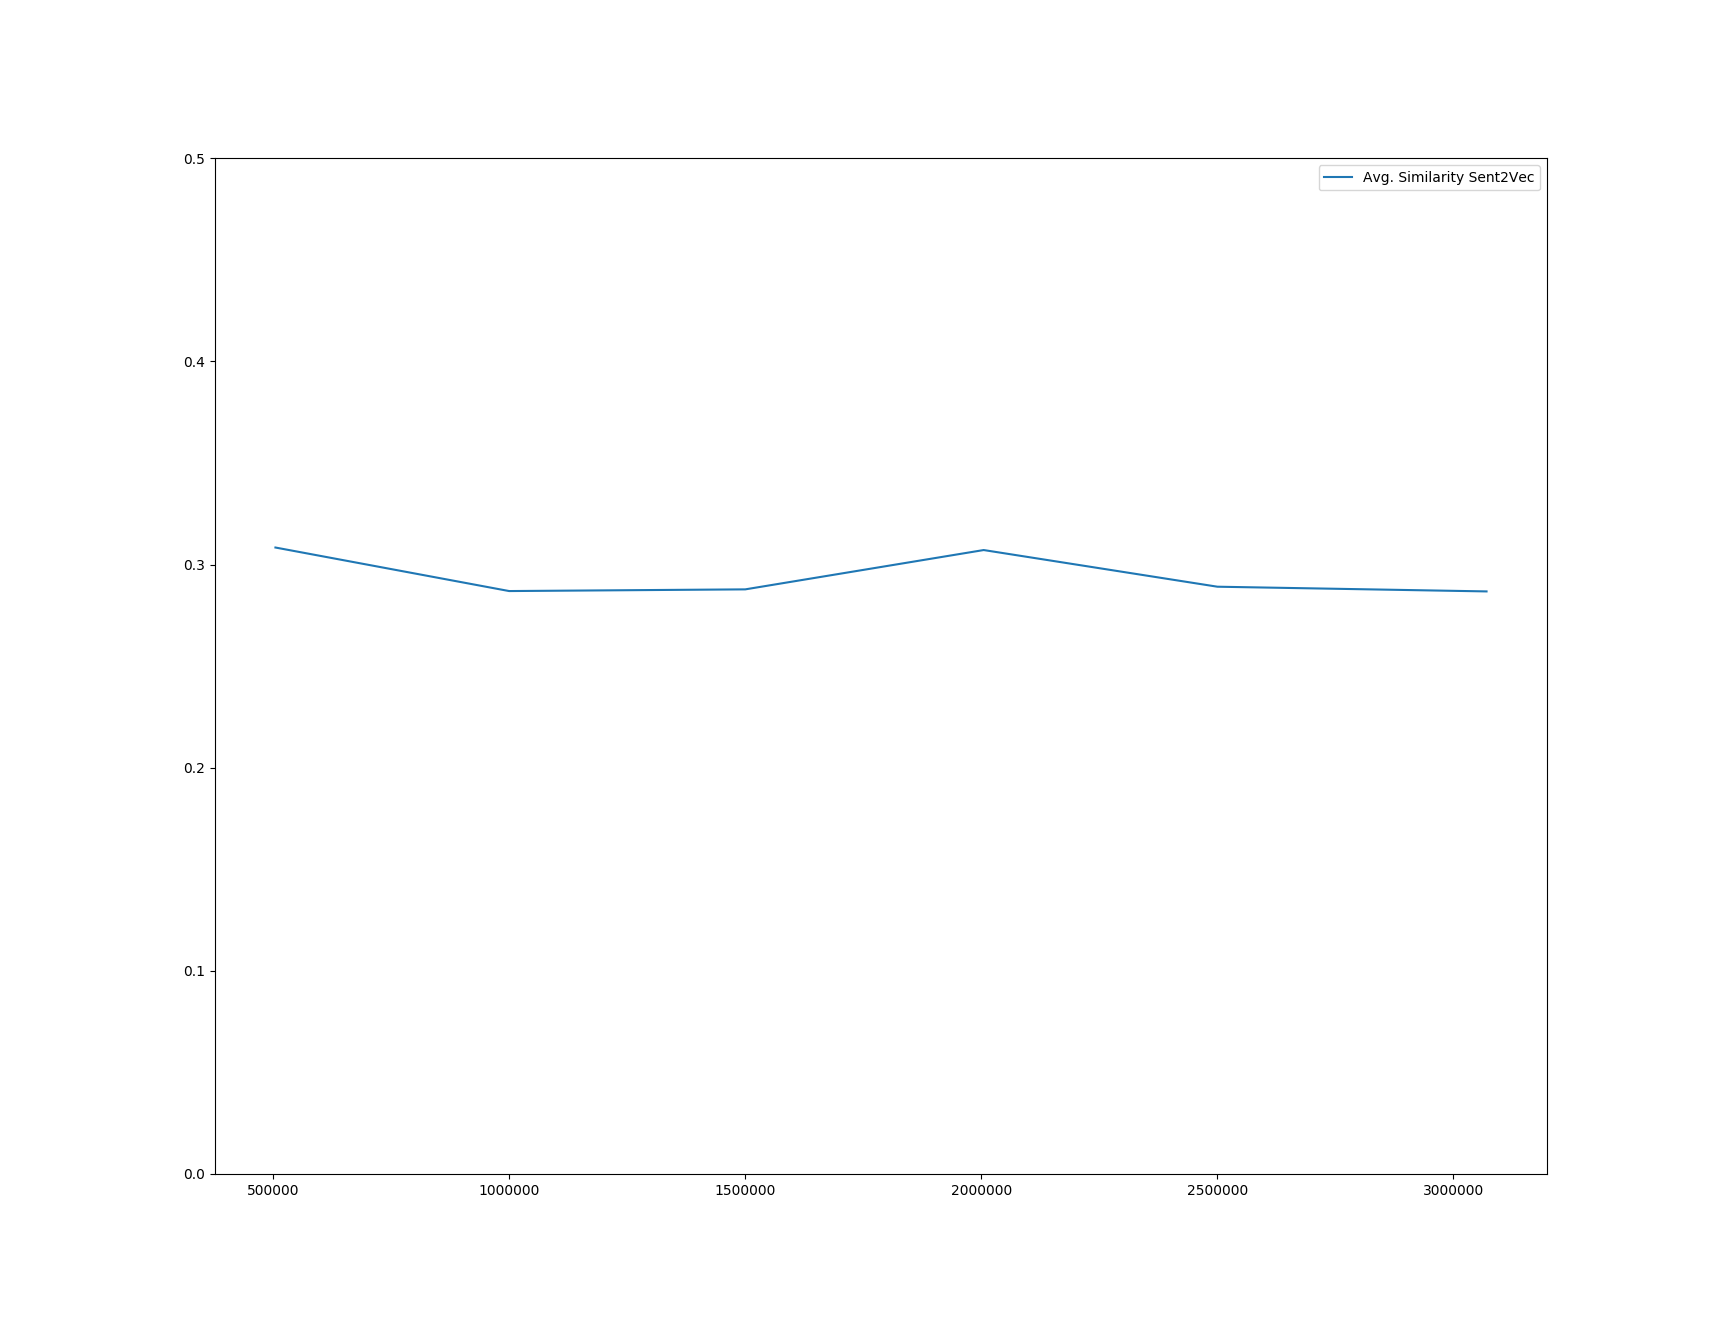
\includegraphics[width=\linewidth]{img/plots/reddit/s2v_twitter_cosine_similarity.png}
	\centering
	\small
	\text{Twitter}
	\endminipage\hfill
	\caption{Results of the evaluation with Sent2Vec on the outputs of the Reddit models using the pretrained models. The ticks on the x-axis show the different snapshots and the y-axis the average semantic similarity when using Sent2Vec for each snapshot.}
	\label{results:sent2vec:reddit:results}
\end{figure}
\begin{table}[H]
	\centering
	\ra{1.3}
	\begin{adjustbox}{max width=\textwidth}
		\begin{tabular}{lcc}
			\toprule
			Snapshot & Avg. Similarity (Wikipedia) & Avg. Similarity (Twitter)\\
			\midrule
			0.5M & $0.33691$ & $0.30837$\\
			1.0M & $0.33689$ & $0.28694$\\
			1.5M & $0.35340$ & $0.28777$\\
			2.0M & $0.33843$ & $0.30713$\\
			2.5M & $0.35828$ & $0.28908$\\
			3.0M & $0.35956$ & $0.28676$\\
			\bottomrule
		\end{tabular}
	\end{adjustbox}
	\caption{The average similarities when applying the Sent2Vec metric on the expected and generated responses from the Reddit model.}
	\label{results:sent2vec:reddit:results_table}
\end{table}

\paragraph{Generic Response are a Problem} One potential reason for the bad results when using the Sent2Vec metric is that we witnessed both models generating generic responses a lot of the time. To analyze this our first idea was to see, what kind of sentences the models produce with the inputs of the test datasets. We did an analysis on the generated responses and quickly noticed that there are a few sentences, which the models predict a lot of time (see Tables~\ref{results:test_performance:opensubtitles_sample_outputs} and~\ref{results:test_performance:reddit_sample_outputs}).\todo{name percentages of tables}
\\
\begin{table}[H]
	\centering
	\ra{1.3}
	\begin{adjustbox}{max width=\textwidth}
		\begin{tabular}{ll}
			\toprule
			Sentence & Frequency\\ \midrule
			\texttt{i m not gon na let you go} & 41853\\
			\texttt{i m not sure i can trust you} & 21263\\
			\texttt{i m not gon na say anything} & 9163\\
			\texttt{i m not gon na let that happen} & 7426\\
			\texttt{i m sorry} & 7235\\
			\texttt{you re not gon na believe this} & 7068\\
			\texttt{you re not gon na believe me} & 6878\\
			\texttt{i m not gon na hurt} you & 4829\\
			\texttt{i m not a fan} & 4468\\
			\texttt{i m not sure} & 4215\\
			\bottomrule
		\end{tabular}
	\end{adjustbox}
	\caption{Top 10 most generated responses with respective occurence frequencies when using the last OpenSubtitles snapshot on the test dataset.}
	\label{results:test_performance:opensubtitles_sample_outputs}
\end{table}\todo{Prozent von Ouptuts als spalte pro satz}\todo{make tables the same width!}

\begin{table}[H]
	\centering
	\ra{1.3}
	\begin{adjustbox}{max width=\textwidth}
		\begin{tabular}{ll}
			\toprule
			Sentence & Frequency\\ \midrule
			\texttt{i m not sure if i m being sarcastic or not .} & 17486\\
			\texttt{i think it s a bit of a stretch .} & 13058\\
			\texttt{i m not sure if you re being sarcastic or not .} & 11647\\
			\texttt{i m not sure if i m a <unknown> or not .} & 8307\\
			\texttt{i m not sure if you re joking or not .} & 7932\\
			\texttt{i was thinking the same thing .} & 7579\\
			\texttt{<unknown>} & 6210\\
			\texttt{i m not sure if i m going to watch this or not .} & 4257\\
			\specialcell{\texttt{i m not sure if i m a fan of the show , but i m}\\\texttt{pretty sure that s a <unknown> .}} & 3232\\
			\texttt{i m not sure if i m going to watch it or not .} & 3079\\
			\bottomrule
		\end{tabular}
	\end{adjustbox}
	\caption{Top 10 most generated sentences with respective occurence frequencies when using the last Reddit snapshot on the test dataset.}
	\label{results:test_performance:reddit_sample_outputs}
\end{table}\todo{Prozent von Ouptuts als spalte pro satz}\todo{make tables the same width!}

\paragraph{Does Filtering of Generic Responses Help?} As seen in the both tables above, there are certain responses which are generated a lot of time and are pretty generic and meaningless. Because of that, we thought it would be a good idea to evaluate the models under the Sent2Vec metric one more time, but this time with the top $n$ generic sentences filtered out. We did this with the hope that the generic sentences are the cause of the small average similarities. The results of the analysis with the top $n$ sentences filtered out can be found in Table~\ref{results:sent2vec:opensubtitles:top_n_results_table} and~\ref{results:sent2vec:reddit:top_n_results_table}. For this analysis, we have only used the Wikipedia model as it has shown a better performance for both of our models before.
\\
\begin{table}[H]
	\centering
	\ra{1.3}
	\begin{adjustbox}{max width=\textwidth}
		\begin{tabular}{lccc}
			\toprule
			Snapshot & $n = 1$ & $n = 5$ & $n = 10$\\
			\midrule
			0.5M & $0.16679$ & $0.16804$ & $0.16854$\\
			1.0M & $0.19329$ & $0.19394$ & $0.19575$\\
			1.5M & $0.19491$ & $0.19519$ & $0.19539$\\
			2.0M & $0.19215$ & $0.19192$ & $0.19284$\\
			2.5M & $0.20102$ & $0.20127$ & $0.20182$\\
			3.0M & $0.20431$ & $0.20547$ & $0.20568$\\
			\bottomrule
		\end{tabular}
	\end{adjustbox}
	\caption{The average similarities when applying the Sent2Vec metric on the expected and generated responses on the test dataset when filtering out the top $n$ most generated responses the OpenSubtitles model.}
	\label{results:sent2vec:opensubtitles:top_n_results_table}
\end{table}

\begin{table}[H]
	\centering
	\ra{1.3}
	\begin{adjustbox}{max width=\textwidth}
		\begin{tabular}{lccc}
			\toprule
			Snapshot & $n = 1$ & $n = 5$ & $n = 10$\\
			\midrule
			0.5M & $0.33772$ & $0.34101$ & $0.34589$\\
			1.0M & $0.34225$ & $0.34238$ & $0.34295$\\
			1.5M & $0.35383$ & $0.35605$ & $0.35564$\\
			2.0M & $0.34008$ & $0.34009$ & $0.34198$\\
			2.5M & $0.35937$ & $0.36142$ & $0.36175$\\
			3.0M & $0.36043$ & $0.35950$ & $0.36313$\\
			\bottomrule
		\end{tabular}
	\end{adjustbox}
	\caption{The average similarities when applying the Sent2Vec metric on the expected and generated responses on the test dataset when filtering out the top $n$ most generated responses for the Reddit model.}
	\label{results:sent2vec:reddit:top_n_results_table}
\end{table}

As seen in the tables above, the filtering of the most used responses does not help a lot when it comes to the Sent2Vec evaluation.\todo{Maybe one more sentence? Maybe say that metric should be applied to ther models (e.g. Google Paper) to see if we are really that bad or if it is inheritent to the metrics itself}

\paragraph{Mixed Feelings about Performance Metrics} As seen in this chapter, the performance metrics used to evaluate the models tell us a mixed story about the resulting models. On one hand, we see that the training went fine and the learning process run as expected. However, when we then test these trained models against the test datasets with the different metrics, it looks like the performance got worse and worse over the time of the training. This is not true in our subjective opinion after ``talking'' to both models for a prolonged period of time. We think the biggest problem for the evaluation are the generic responses both models seem to generate much more than actual answers. To find the cause of this generic responses, we will now try to analyze the language model which both models have learned while training and try to establish a connection between the language model in the datasets and the ones produced by the models.

\section{Language Model}
As said at the end of the previous chapter, in this chapter we are going to investigate into the language models the trained models produce and try to get a grasp on how much semantic understanding the models have. For the first analysis, we are going to create compare n-gram distributions over the datasets and compare them with the distributions found in the responses when evaluating the models. We also take a look at the most use n-grams to find a reason why the models produce so much generic sentences. After that, we are going to investigate into how the models actually process the input sequences by first taking a look at the generated thought vectors. We will then go on and try to evaluate if the attention mechanism (see Chapter~\ref{fundamentals:soft_attention}) really helps the models when producing responses.\todo{Move to own chapter!}

\paragraph{Uni- and Bigram Distributions over Time}
As the first step, we are going to compare the uni- and bigram distributions of the training datasets with the distributions produced when evaluating the models with the test datasets. For this purpose, we generated unigram and bigram statistics using \texttt{nltk} over the training datasets and outputs generated by the models.

First, let us analyze the bigram distributions which can be seen in the Figures~\ref{results:bigram:distributions:opensubtitles} and~\ref{results:bigram:distributions:reddit}. As seen there, at the beginning of the training (i.e. snapshots 0.5M), the bigrams are distributed pretty evenly. However, as longer as the training continues the more right-leaning the distributions of the bigrams in the outputs of the models get. This seems to coincide with the results found in the previous chapter, that the models start to use less and less bigrams but simultaneously increases the usage frequency of often used bigrams. It is also understandable from a stand point that the models learn, which are the important bigrams and which are not. This is especially apparent in the case of the OpenSubtitles model, where we also witness a big discrepancy between the expected and the generated distributions. However, the development of the distribution in the case of the Reddit model looks quite different. It also becomes more right-leaning as the training advances, but it much better fits the expected distribution, for example bigrams in the snapshot 1.5M have almost the same distribution as in the training data.

\begin{figure}[H]
	\minipage{0.5\textwidth}
	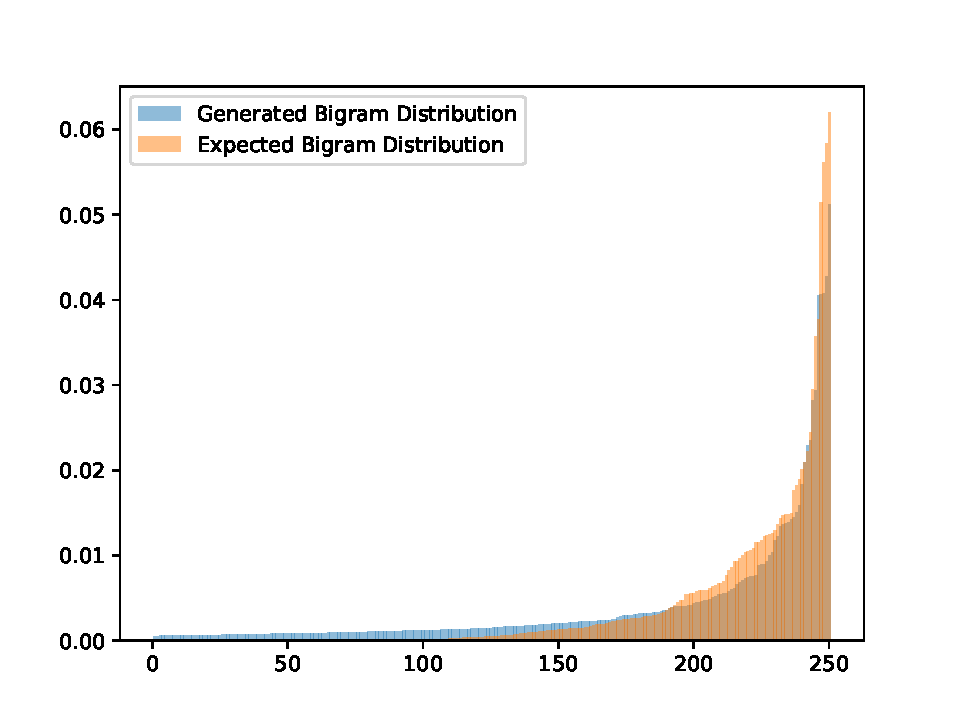
\includegraphics[width=\linewidth]{img/plots/opensubtitles_not_reversed/bigram_distribution_comparison_step_500000.pdf}
	\centering
	\small
	\text{Snapshot 0.5M}
	\endminipage\hfill
	\minipage{0.5\textwidth}
	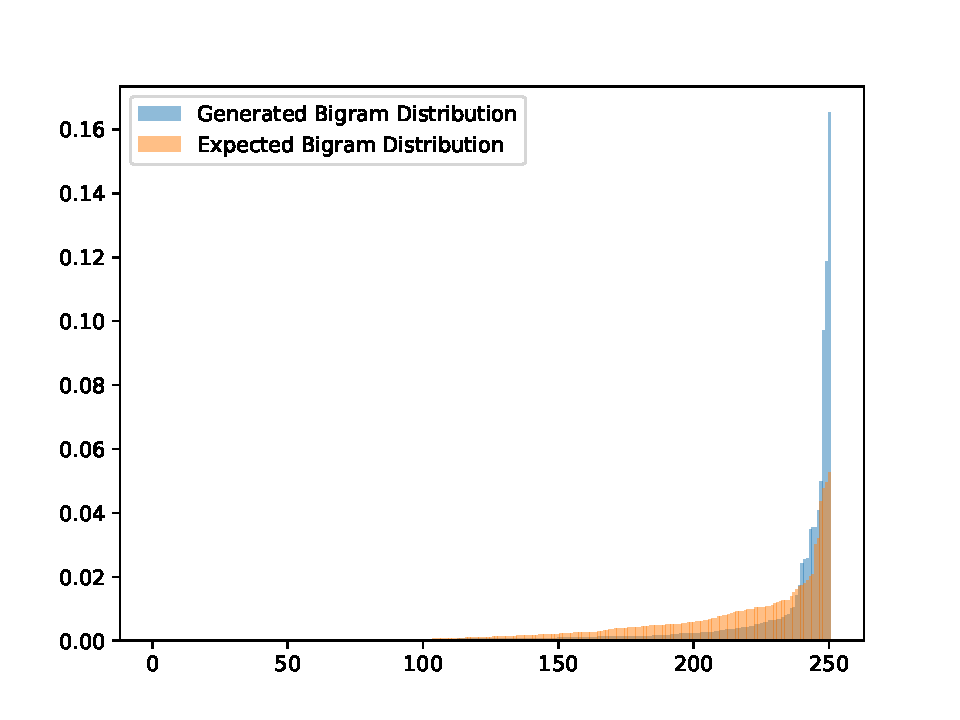
\includegraphics[width=\linewidth]{img/plots/opensubtitles_not_reversed/bigram_distribution_comparison_step_1000000.pdf}
	\centering
	\small
	\text{Snapshot 1.0M}
	\endminipage\hfill
	\minipage{0.5\textwidth}
	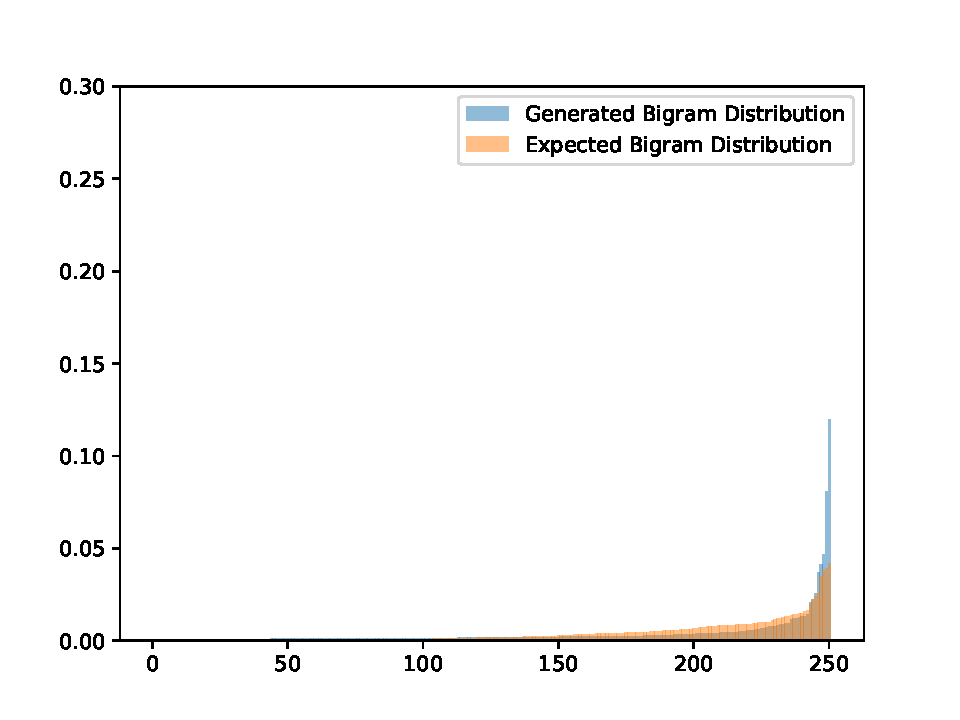
\includegraphics[width=\linewidth]{img/plots/opensubtitles_not_reversed/bigram_distribution_comparison_step_1500000.pdf}
	\centering
	\small
	\text{Snapshot 1.5M}
	\endminipage\hfill
	\minipage{0.5\textwidth}
	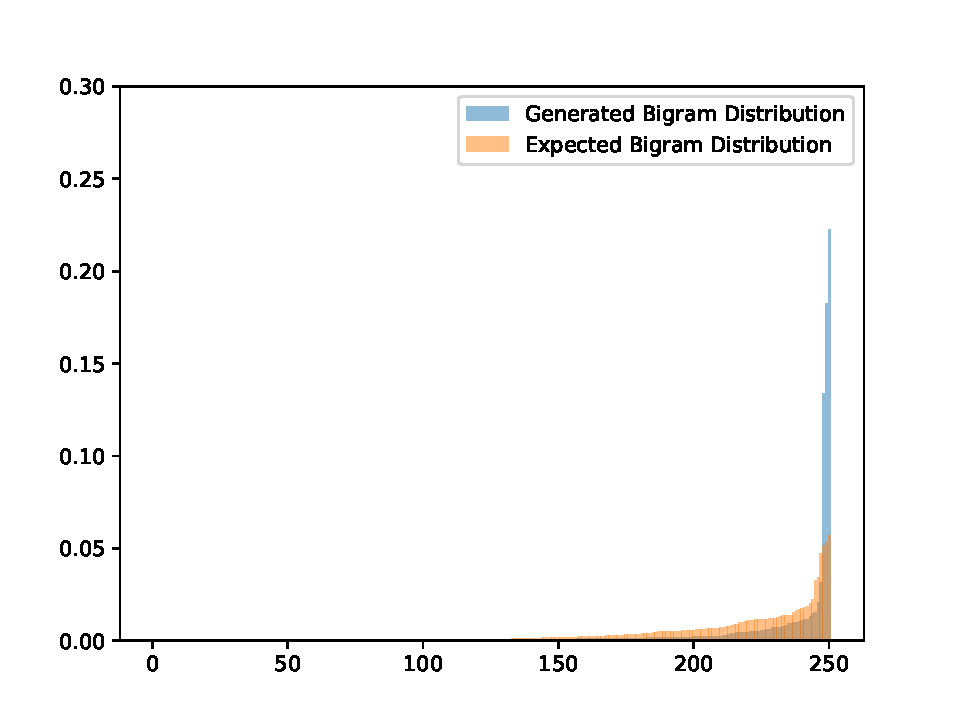
\includegraphics[width=\linewidth]{img/plots/opensubtitles_not_reversed/bigram_distribution_comparison_step_2000000.pdf}
	\centering
	\small
	\text{Snapshot 2.0M}
	\endminipage\hfill
	\minipage{0.5\textwidth}
	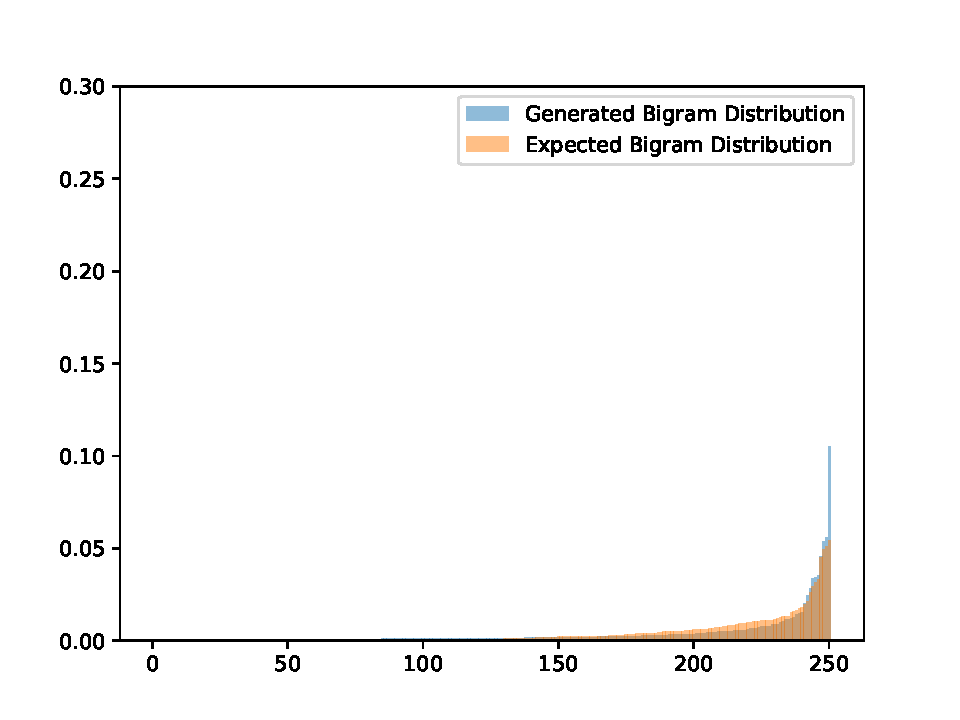
\includegraphics[width=\linewidth]{img/plots/opensubtitles_not_reversed/bigram_distribution_comparison_step_2500000.pdf}
	\centering
	\small
	\text{Snapshot 2.5M}
	\endminipage\hfill
	\minipage{0.5\textwidth}
	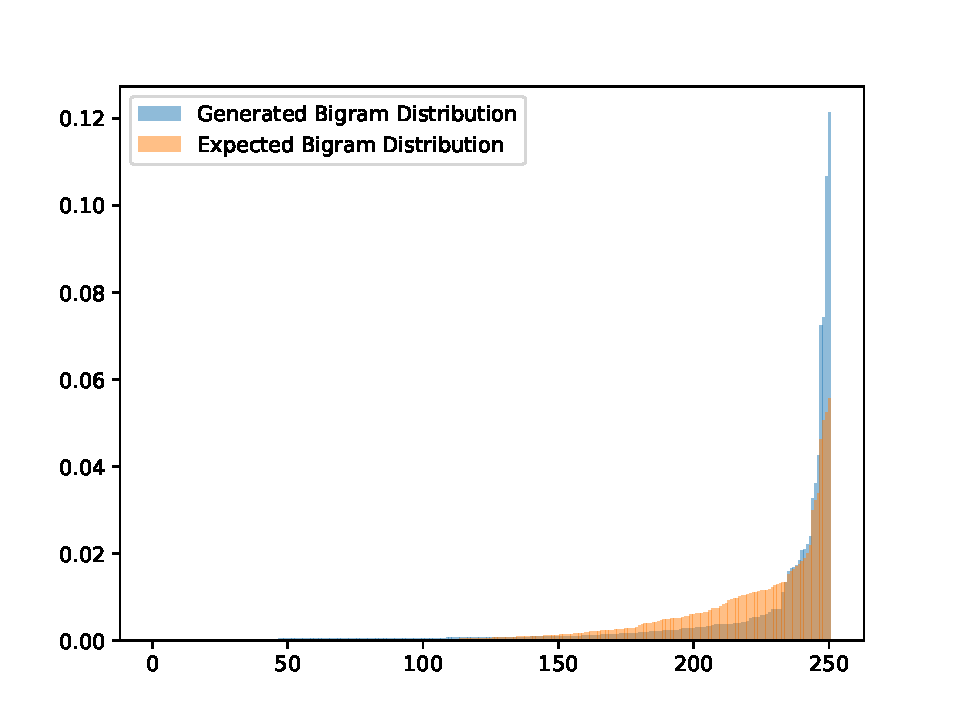
\includegraphics[width=\linewidth]{img/plots/opensubtitles_not_reversed/bigram_distribution_comparison_step_3000000.pdf}
	\centering
	\small
	\text{Snapshot 3.0M}
	\endminipage\hfill
	\caption{Comparison of the distributions of the top 100 most used bigrams for the responses of the OpenSubtitles models (orange) when using the test dataset and the distribution within the training data (blue). The distributions are compared for each snapshot available.}
	\label{results:bigram:distributions:opensubtitles}
\end{figure}

\begin{figure}[H]
	\minipage{0.5\textwidth}
	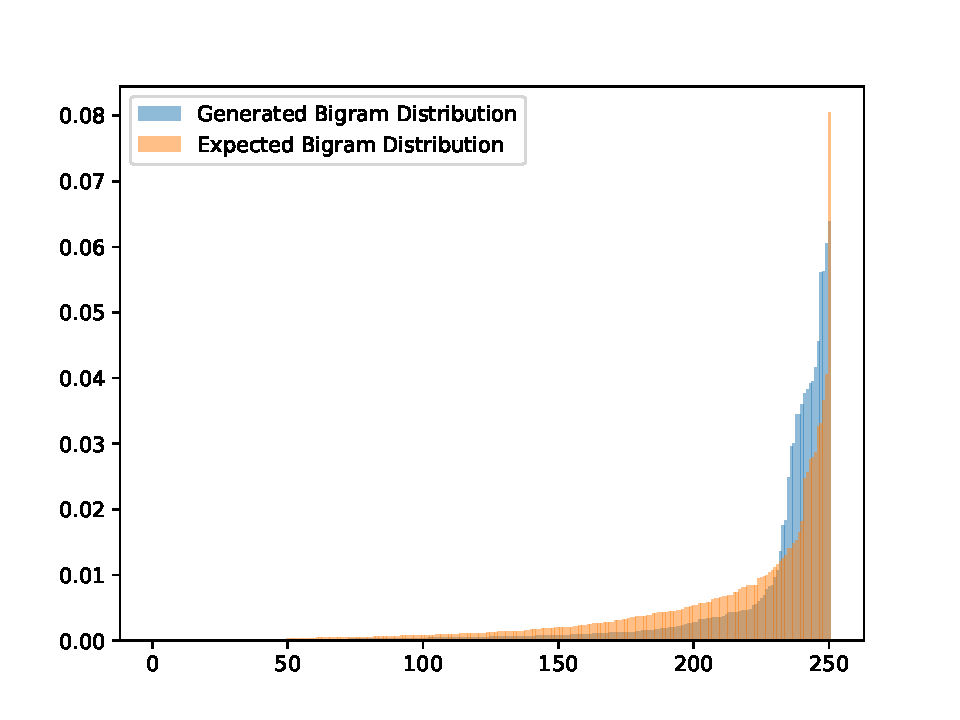
\includegraphics[width=\linewidth]{img/plots/reddit/bigram_distribution_comparison_step_500000.pdf}
	\centering
	\small
	\text{Snapshot 0.5M}
	\endminipage\hfill
	\minipage{0.5\textwidth}
	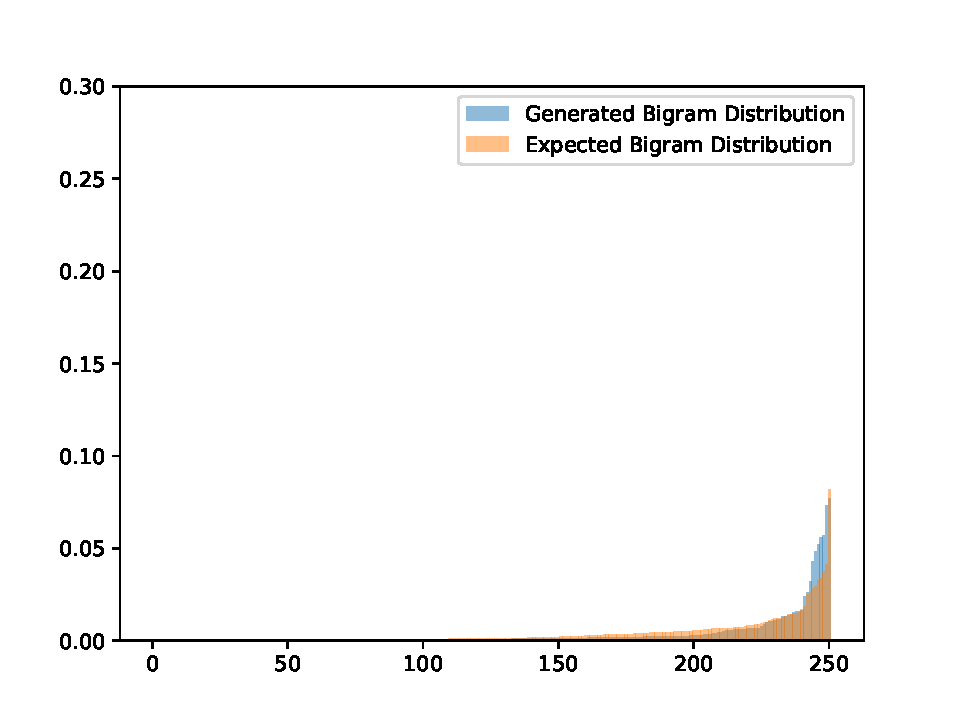
\includegraphics[width=\linewidth]{img/plots/reddit/bigram_distribution_comparison_step_1000000.pdf}
	\centering
	\small
	\text{Snapshot 1.0M}
	\endminipage\hfill
	\minipage{0.5\textwidth}
	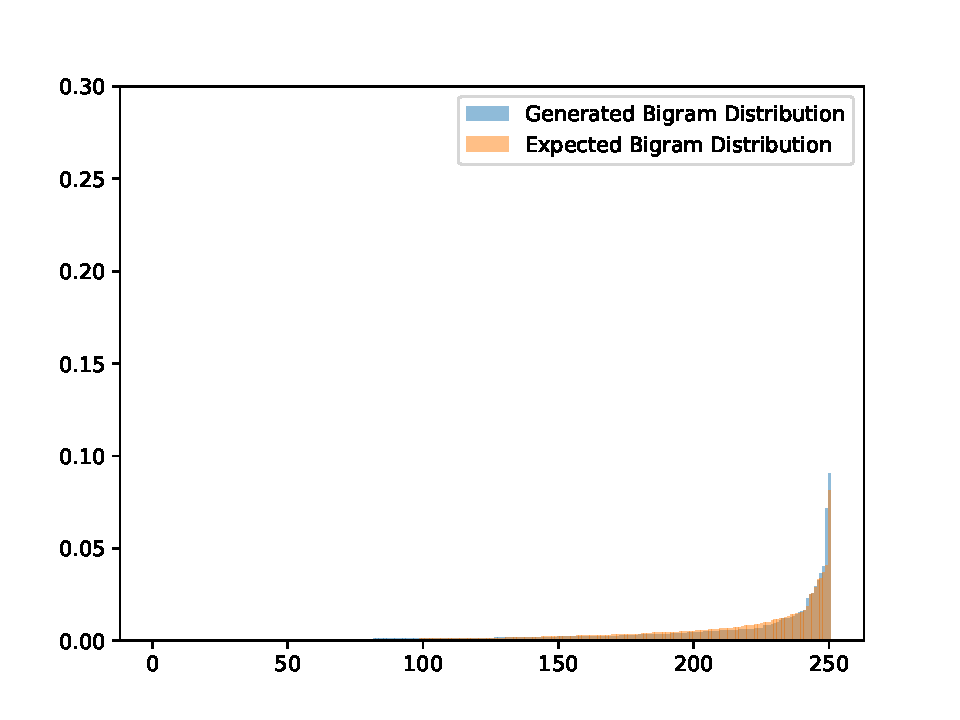
\includegraphics[width=\linewidth]{img/plots/reddit/bigram_distribution_comparison_step_1500000.pdf}
	\centering
	\small
	\text{Snapshot 1.5M}
	\endminipage\hfill
	\minipage{0.5\textwidth}
	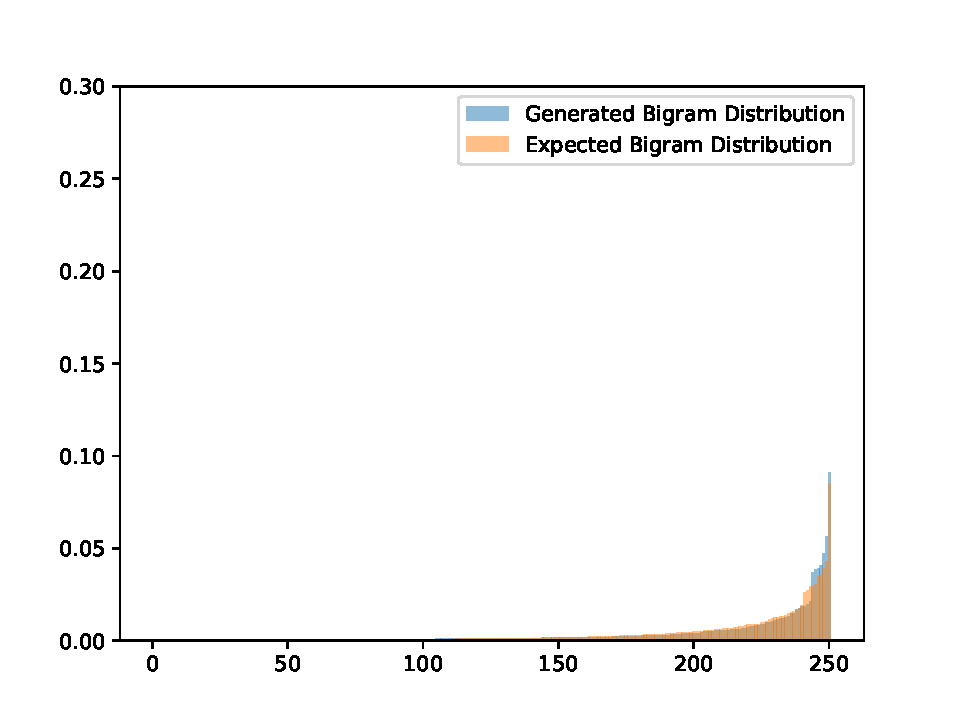
\includegraphics[width=\linewidth]{img/plots/reddit/bigram_distribution_comparison_step_2000000.pdf}
	\centering
	\small
	\text{Snapshot 2.0M}
	\endminipage\hfill
	\minipage{0.5\textwidth}
	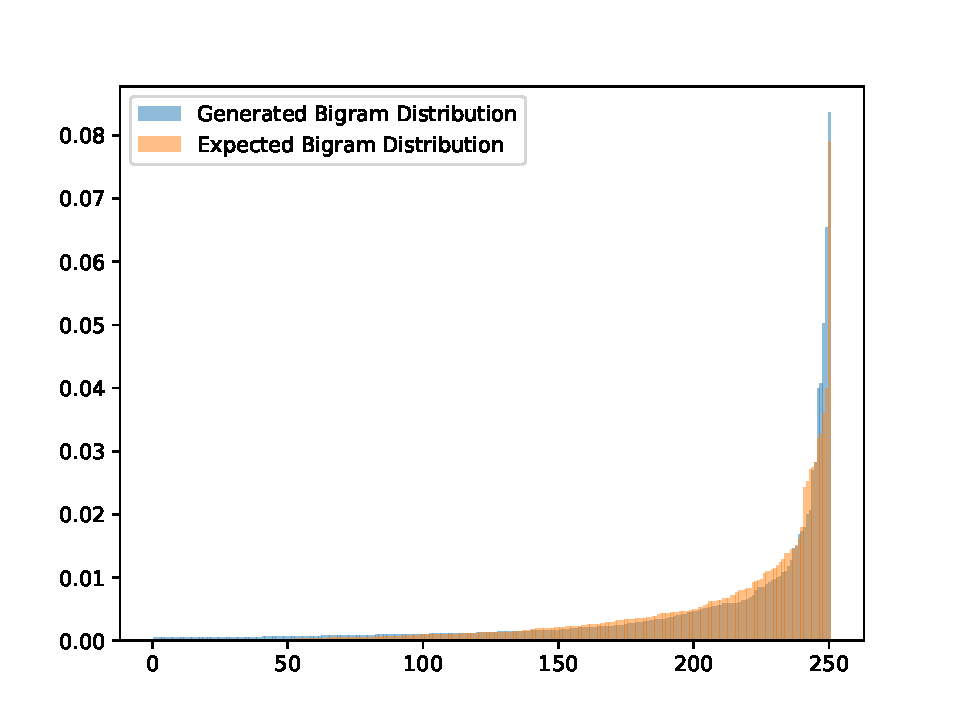
\includegraphics[width=\linewidth]{img/plots/reddit/bigram_distribution_comparison_step_2500000.pdf}
	\centering
	\small
	\text{Snapshot 2.5M}
	\endminipage\hfill
	\minipage{0.5\textwidth}
	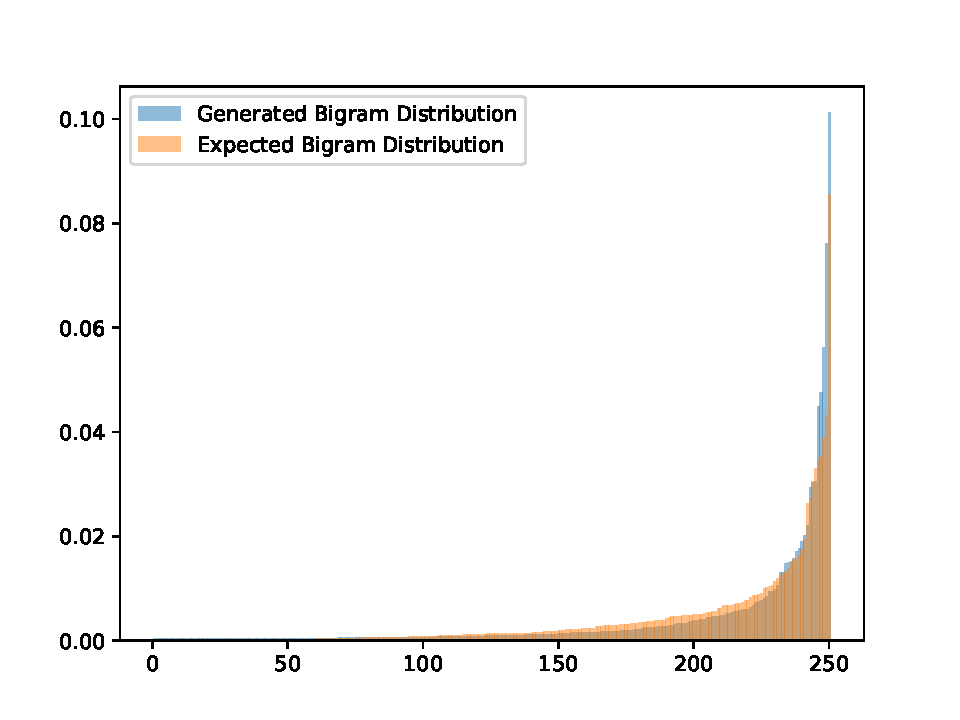
\includegraphics[width=\linewidth]{img/plots/reddit/bigram_distribution_comparison_step_3000000.pdf}
	\centering
	\small
	\text{Snapshot 3.0M}
	\endminipage\hfill
	\caption{Comparison of the distributions of the top 100 most used bigrams for the responses of the Reddit models (orange) when using the test dataset and the distribution within the training data (blue). The distributions are compared for each snapshot available.}
	\label{results:bigram:distributions:reddit}
\end{figure}

\begin{figure}[H]
	\minipage{0.5\textwidth}
	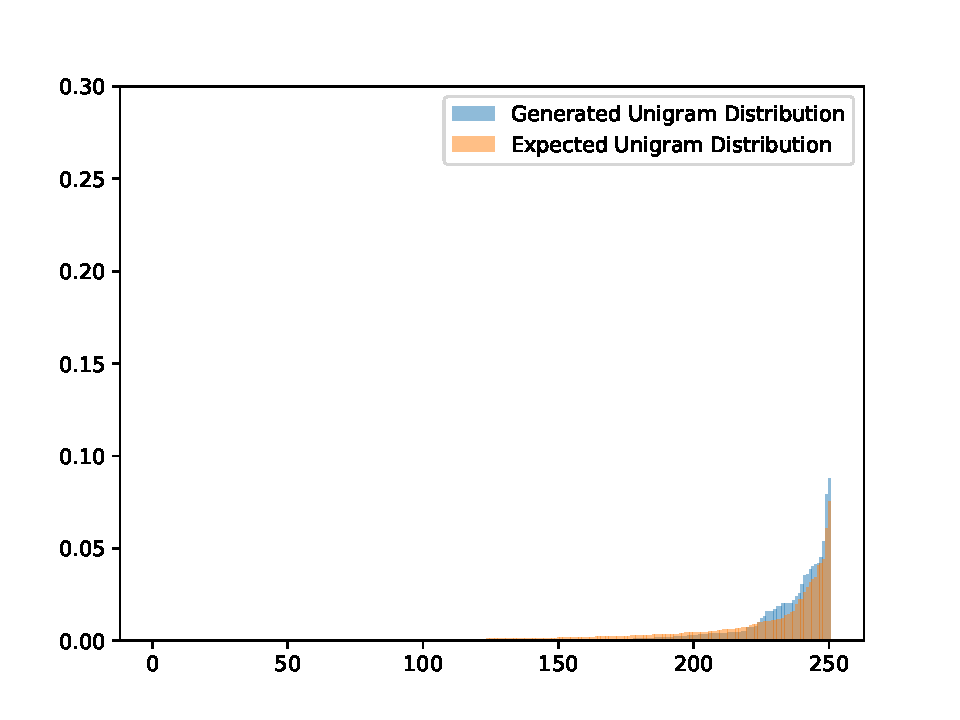
\includegraphics[width=\linewidth]{img/plots/opensubtitles_not_reversed/unigram_distribution_comparison_step_500000.pdf}
	\centering
	\small
	\text{Snapshot 0.5M}
	\endminipage\hfill
	\minipage{0.5\textwidth}
	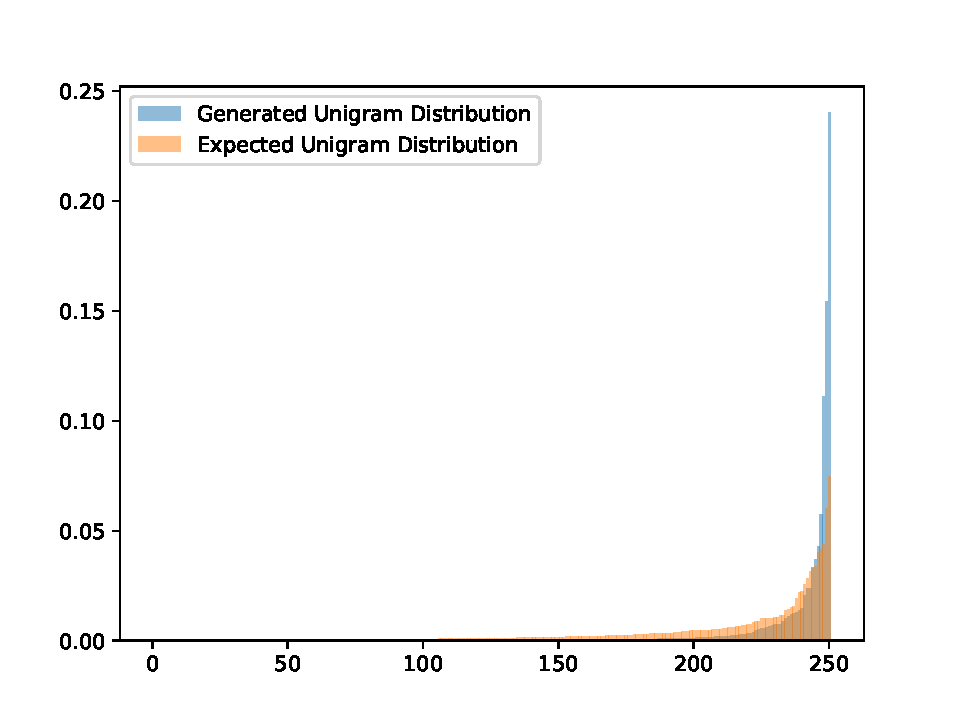
\includegraphics[width=\linewidth]{img/plots/opensubtitles_not_reversed/unigram_distribution_comparison_step_1000000.pdf}
	\centering
	\small
	\text{Snapshot 1.0M}
	\endminipage\hfill
	\minipage{0.5\textwidth}
	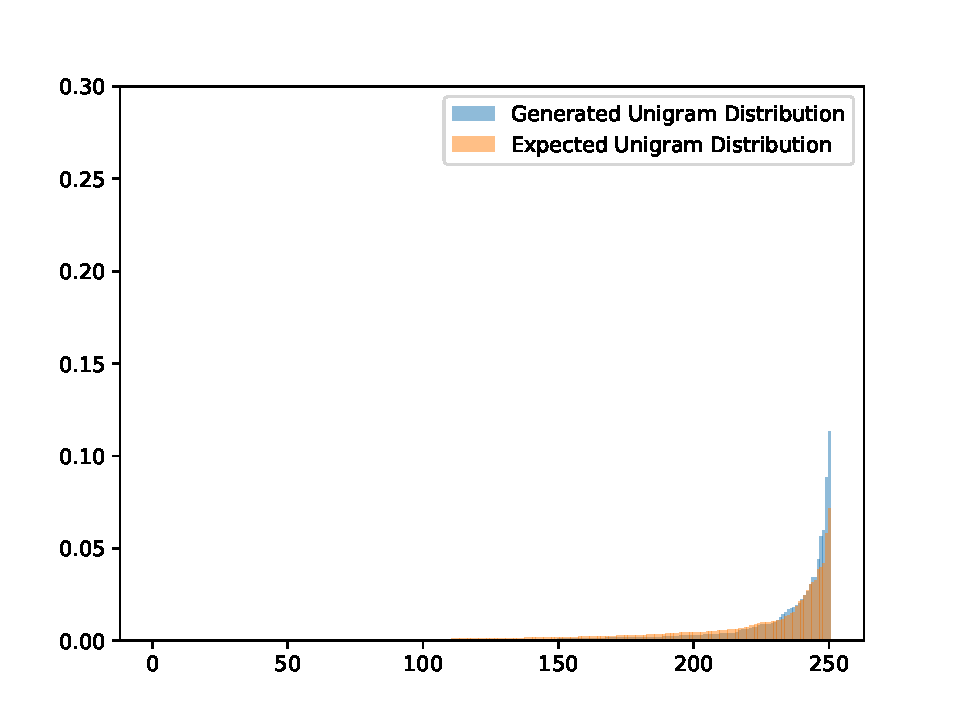
\includegraphics[width=\linewidth]{img/plots/opensubtitles_not_reversed/unigram_distribution_comparison_step_1500000.pdf}
	\centering
	\small
	\text{Snapshot 1.5M}
	\endminipage\hfill
	\minipage{0.5\textwidth}
	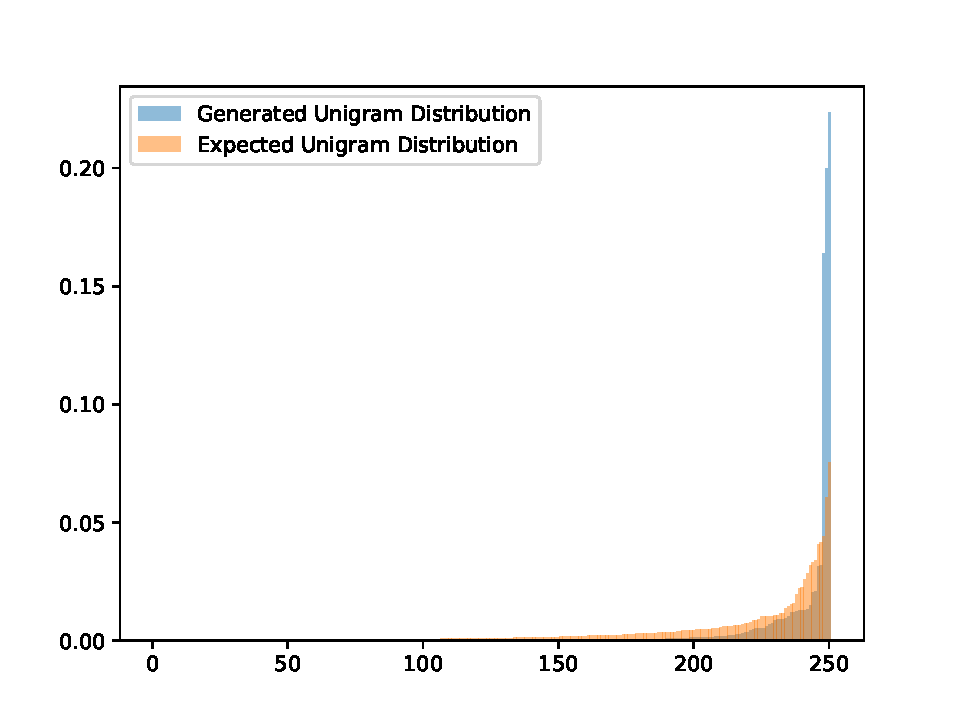
\includegraphics[width=\linewidth]{img/plots/opensubtitles_not_reversed/unigram_distribution_comparison_step_2000000.pdf}
	\centering
	\small
	\text{Snapshot 2.0M}
	\endminipage\hfill
	\minipage{0.5\textwidth}
	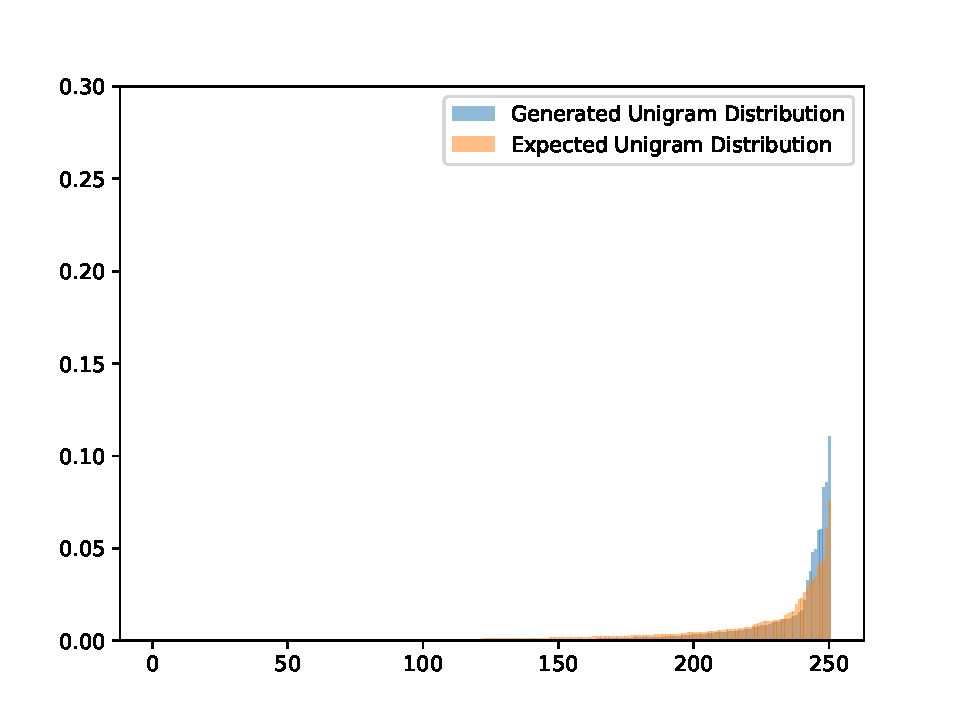
\includegraphics[width=\linewidth]{img/plots/opensubtitles_not_reversed/unigram_distribution_comparison_step_2500000.pdf}
	\centering
	\small
	\text{Snapshot 2.5M}
	\endminipage\hfill
	\minipage{0.5\textwidth}
	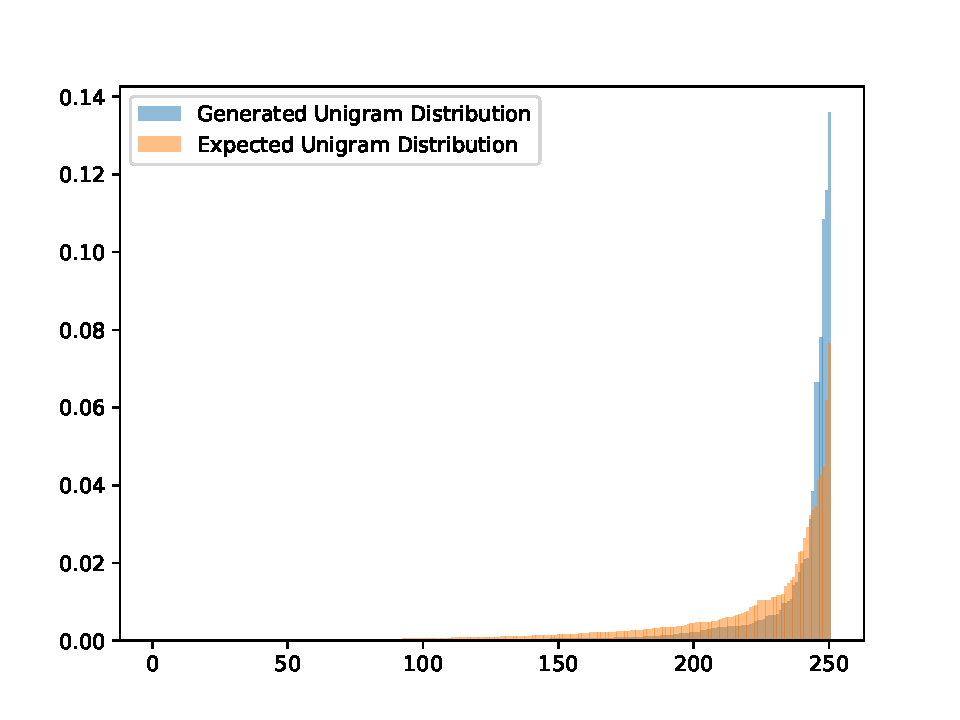
\includegraphics[width=\linewidth]{img/plots/opensubtitles_not_reversed/unigram_distribution_comparison_step_3000000.pdf}
	\centering
	\small
	\text{Snapshot 3.0M}
	\endminipage\hfill
	\caption{Comparison of the distributions of the top 100 most used unigrams for the responses of the OpenSubtitles models (orange) when using the test dataset and the distribution within the training data (blue). The distributions are compared for each snapshot available.}
	\label{results:unigram:distributions:opensubtitles}
\end{figure}

\begin{figure}[H]
	\minipage{0.5\textwidth}
	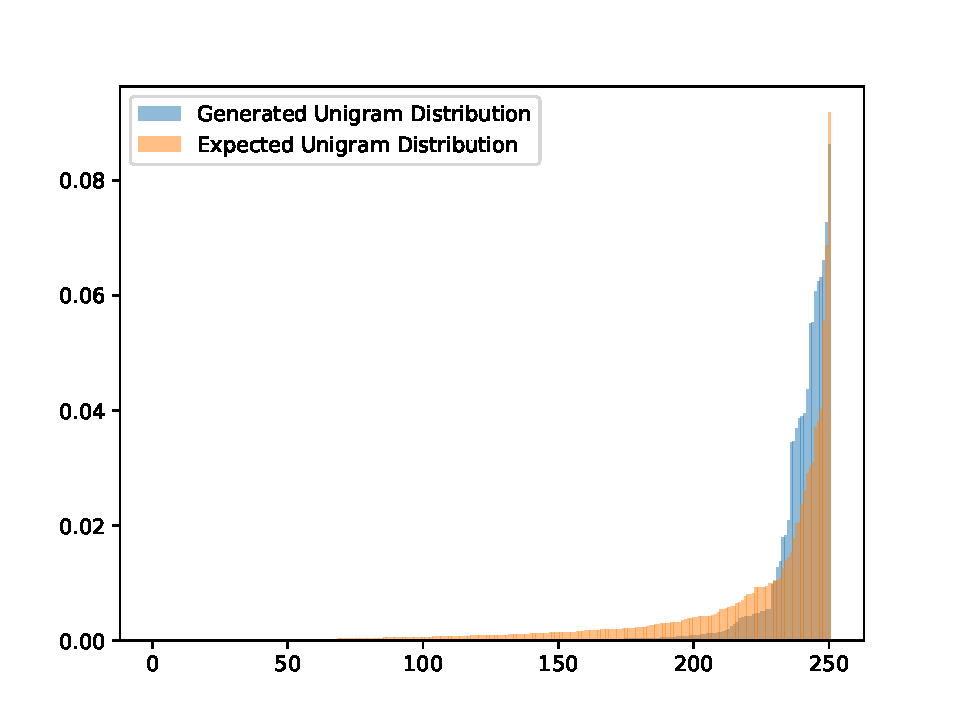
\includegraphics[width=\linewidth]{img/plots/reddit/unigram_distribution_comparison_step_500000.pdf}
	\centering
	\small
	\text{Snapshot 0.5M}
	\endminipage\hfill
	\minipage{0.5\textwidth}
	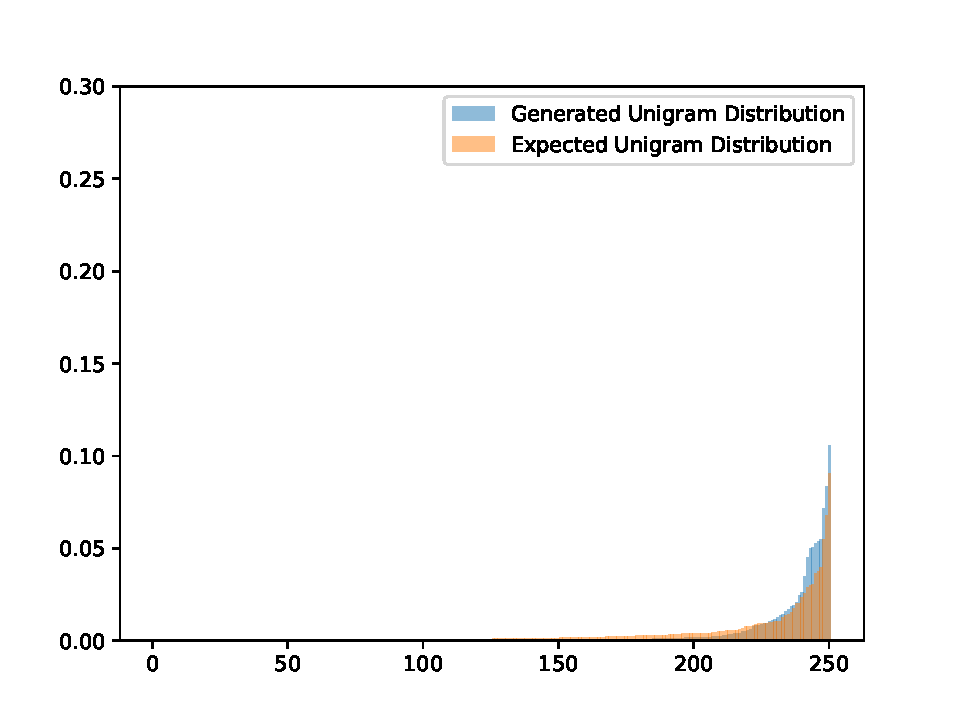
\includegraphics[width=\linewidth]{img/plots/reddit/unigram_distribution_comparison_step_1000000.pdf}
	\centering
	\small
	\text{Snapshot 1.0M}
	\endminipage\hfill
	\minipage{0.5\textwidth}
	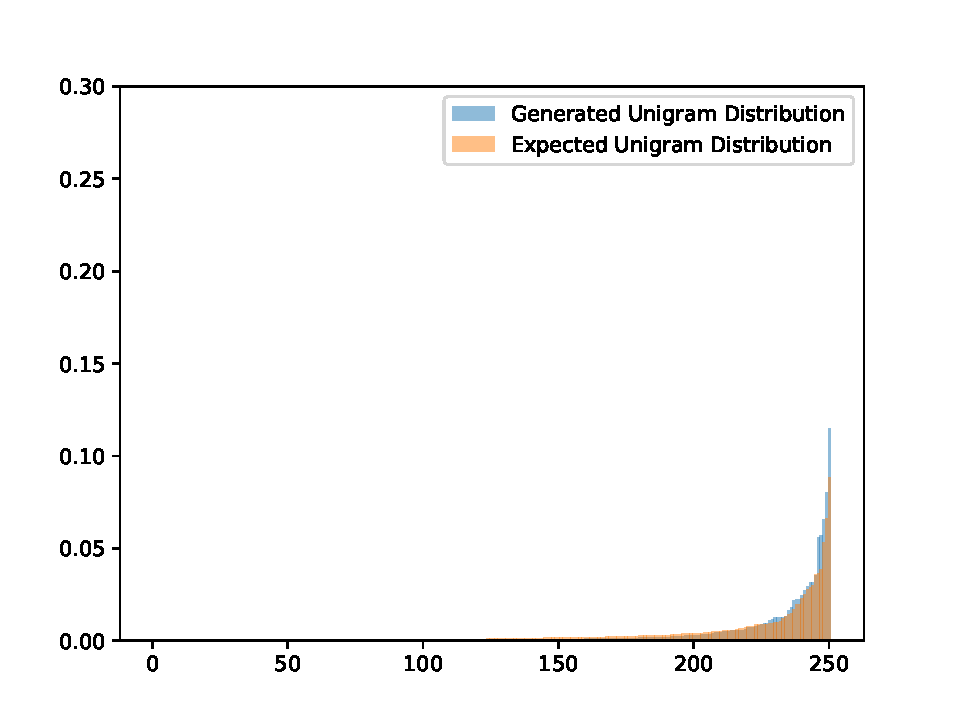
\includegraphics[width=\linewidth]{img/plots/reddit/unigram_distribution_comparison_step_1500000.pdf}
	\centering
	\small
	\text{Snapshot 1.5M}
	\endminipage\hfill
	\minipage{0.5\textwidth}
	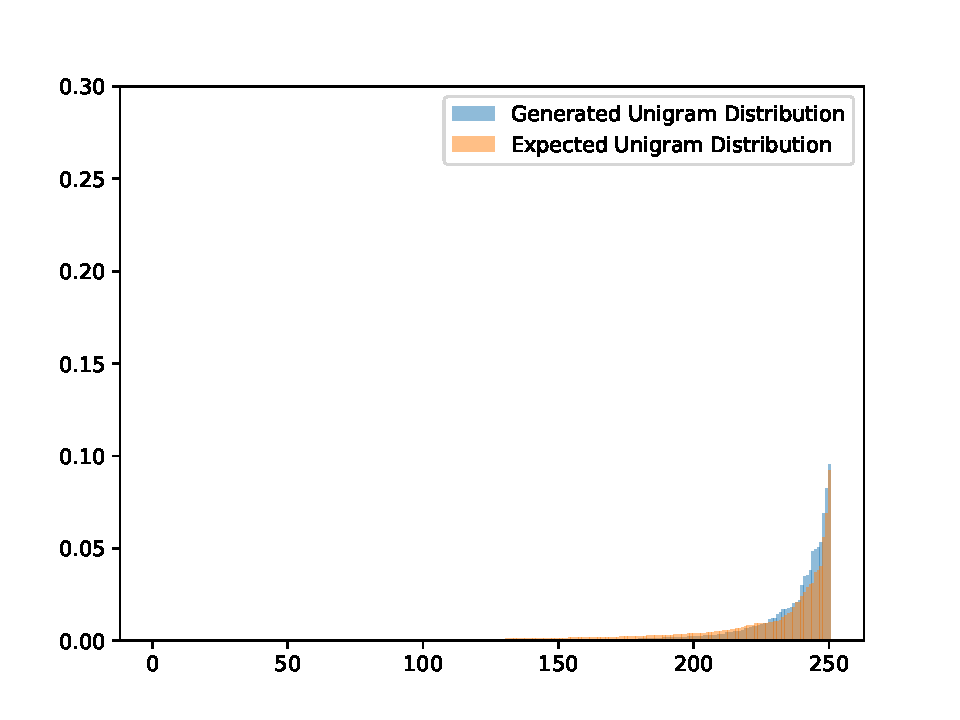
\includegraphics[width=\linewidth]{img/plots/reddit/unigram_distribution_comparison_step_2000000.pdf}
	\centering
	\small
	\text{Snapshot 2.0M}
	\endminipage\hfill
	\minipage{0.5\textwidth}
	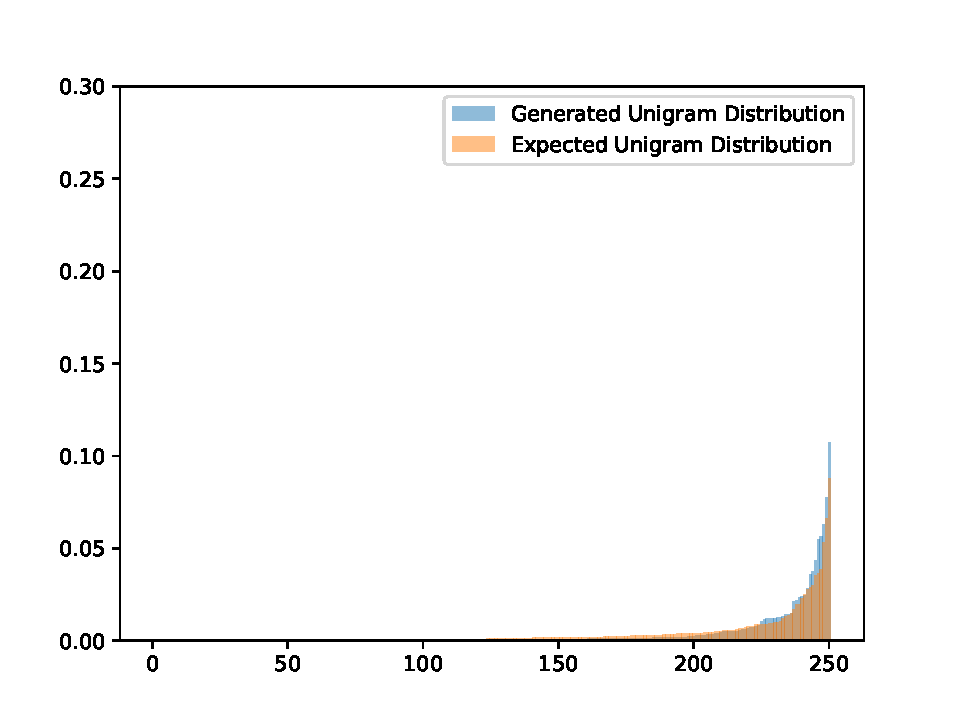
\includegraphics[width=\linewidth]{img/plots/reddit/unigram_distribution_comparison_step_2500000.pdf}
	\centering
	\small
	\text{Snapshot 2.5M}
	\endminipage\hfill
	\minipage{0.5\textwidth}
	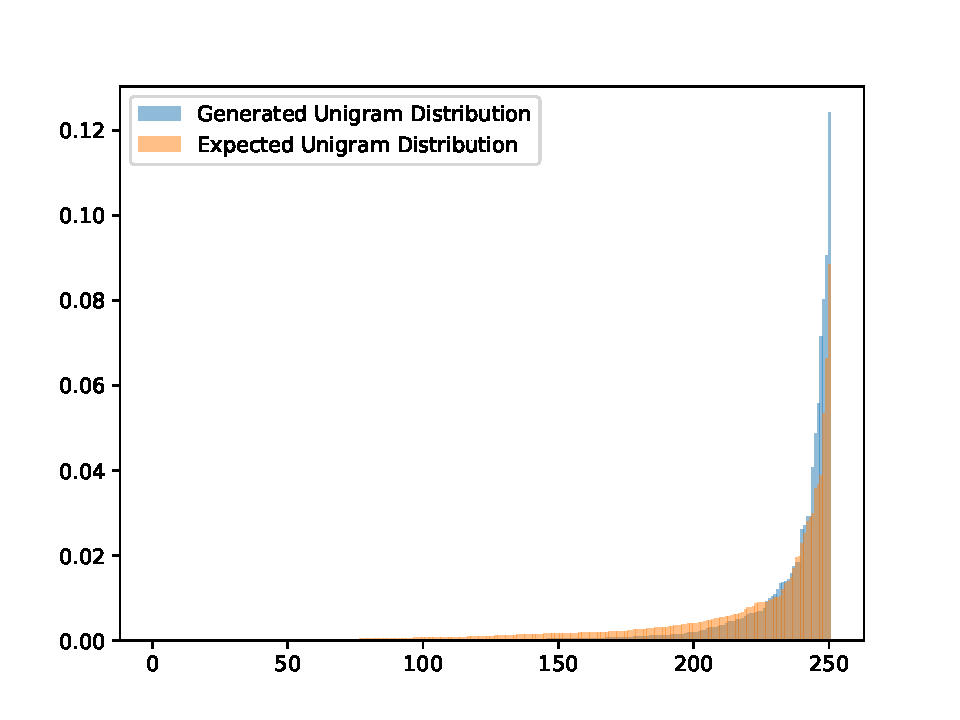
\includegraphics[width=\linewidth]{img/plots/reddit/unigram_distribution_comparison_step_3000000.pdf}
	\centering
	\small
	\text{Snapshot 3.0M}
	\endminipage\hfill
	\caption{Comparison of the distributions of the top 100 most used unigrams for the responses of the Reddit models (orange) when using the test dataset and the distribution within the training data (blue). The distributions are compared for each snapshot available.}
	\label{results:unigram:distributions:reddit}
\end{figure}

\subsection{Bi-Gramm}
In den Grafiken \ref{results:ngram:distributions:opensubtitles} und \ref{results:ngram:distributions:reddit} wird dargestellt (erklären, was genau man sieht, muss genau sein, da nicht ganz einfach.)
\paragraph{Die bi-gramme und deren Wahrscheinlichkeiten werden übernommen.}
\todo{grafiken interpretieren}
\paragraph{The distribution is right-handed} of the words... Für beide Modelle gilt: Starten gleichverteilter, als expected, nähern sich dann dem expected Werten an. Dieser Virgang scheint von links nacht rechts stattzufinden. Das scheint insofern nachvollziehbar, dass er schnell merkt, welche bi-gramme nicht oft vorkommen und entsprechend diese fast nie verwendet.Jedoch herauszufinden, welches der top n n-gramme das Richtige ist, ist ein deutlich schwierigerer Lernprozess. Wir sehen im groben zumindest eine Annäherung der Verteilung. Wünschenswert wäre natürlich hier eine ähnliche Verteilung wie expected, wobei vor allem die weniger häufigen Bigramme für eine vielfältige Sprache stehen. Dies würde sich ganz generell als mass für die Sprachvielfalt eigenen, indem man z.B. die umgekehrte Wahrscheinlichkeit als Gewicht Einfliessen lässt.

\subsection{Uni-gramm/Wörter}
\todo{grafiken erstellen und referenzieren und beschreiben}
\paragraph{Die Uni-gramm und deren Wahrscheinlichkeiten werden übernommen.}
\todo{grafiken interpretieren}
\paragraph{The distribution is}
\todo{grafiken interpretieren}

\paragraph{Thought Vectors for Input Sequences}\todo{move to own chapter at the end} After the encoder has processed the whole input sequences, it pass it forward to the decoder to construct the output sequence (see Chapter~\ref{fundamentals:seq2seq}). It is the only direct connection the encoder and decoder have in such a model, which means, that the encoder has to ``encode'' all the information into this thought vector before passing it to the decoder. The thought vector hence represents an embedding of the input sequence in an $n$ dimensional vector space, where $n$ stands for the size of the thought vector. To analyze this embeddings, we collected them for 15 different sample sentences and projected them via PCA into two dimensional space, the results of this projection can be see in Figure~\ref{results:thougth_vectors:embeddings:opensubtitles} and~\ref{results:thougth_vectors:embeddings:reddit} below.

\begin{figure}[H]
	\centering
	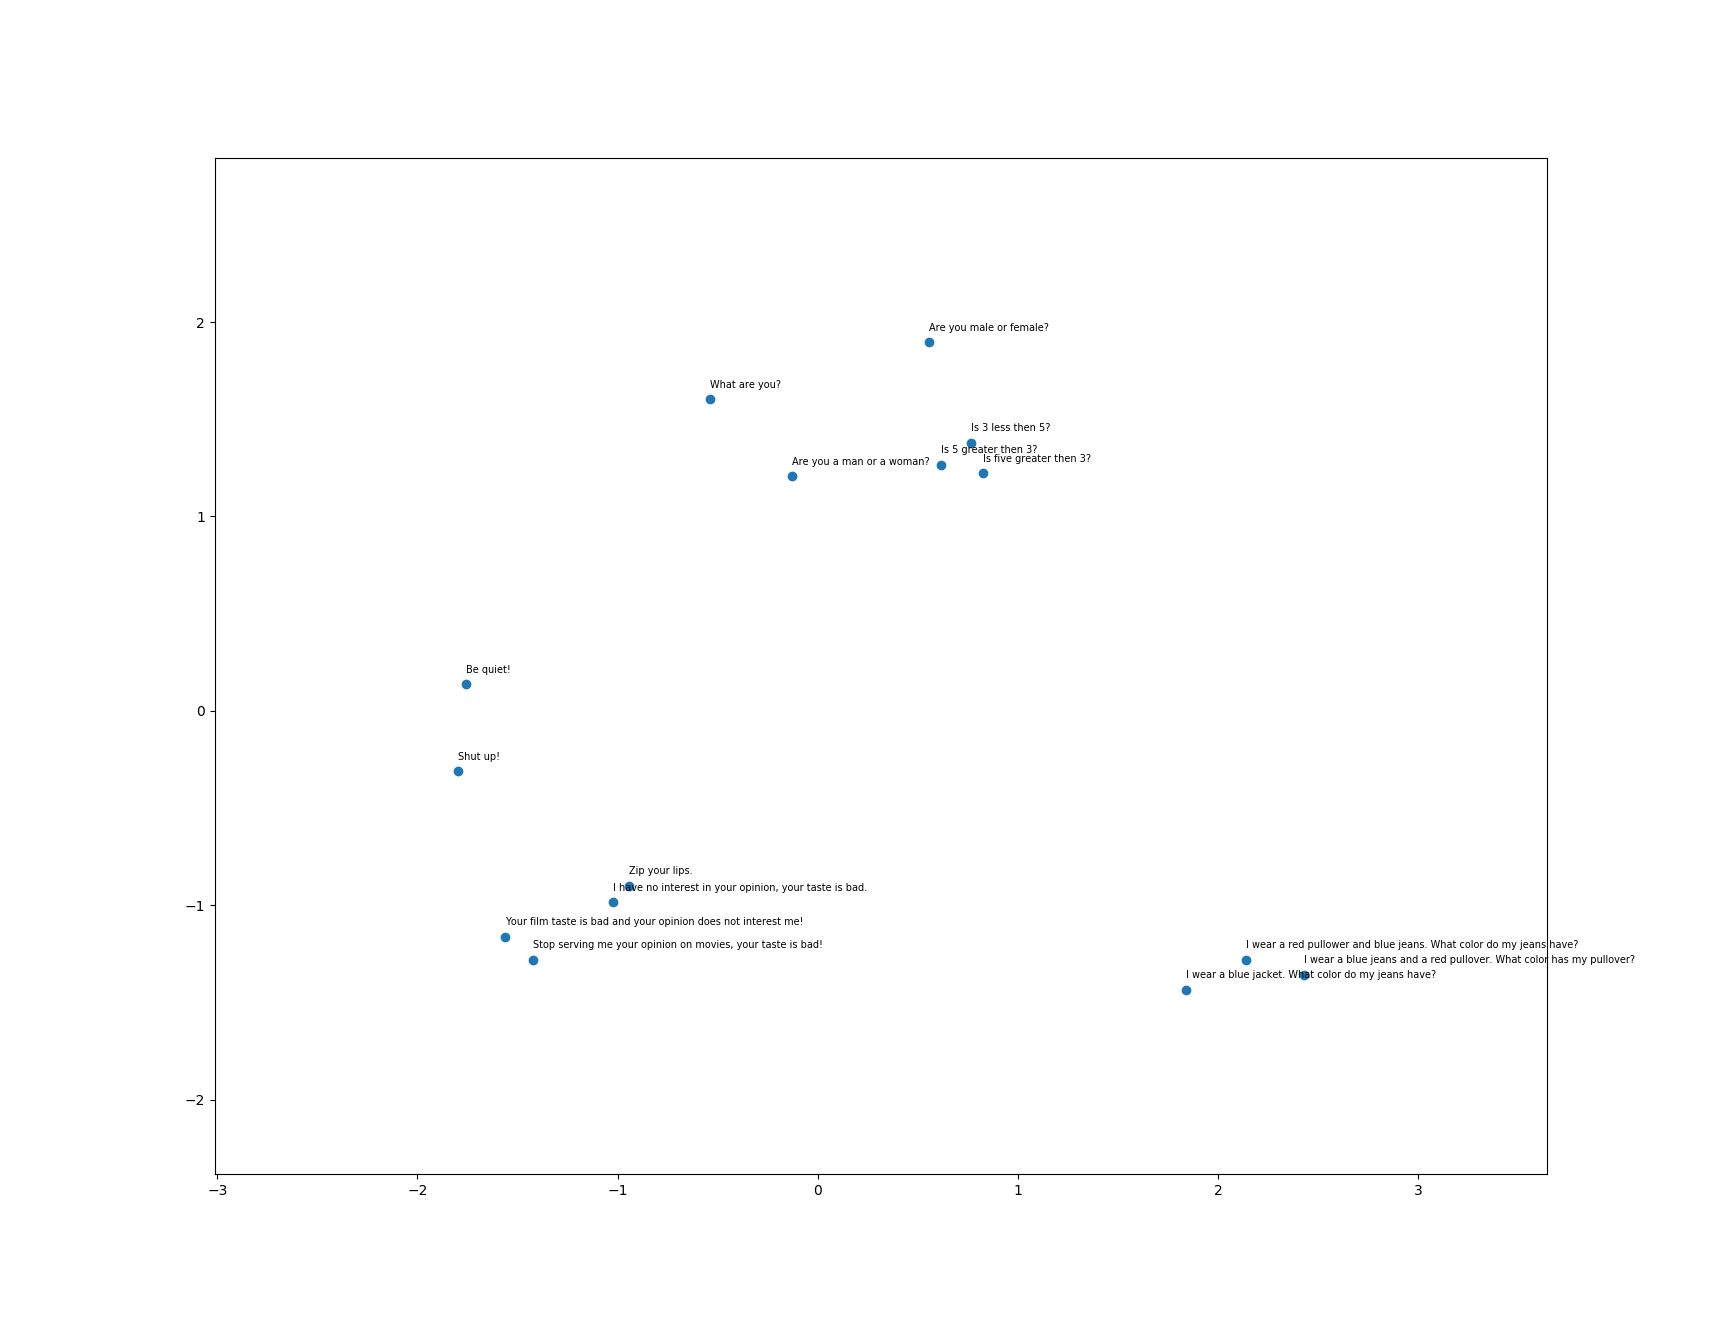
\includegraphics[width=16cm]{img/opensubtitles_thought_vector_embeddings.png}
	\caption{The projected thought vectors for 15 different sentences when using the OpenSubtitles model. PCA was used for the projection.}
	\label{results:thougth_vectors:embeddings:opensubtitles}
\end{figure}

\begin{figure}[H]
	\centering
	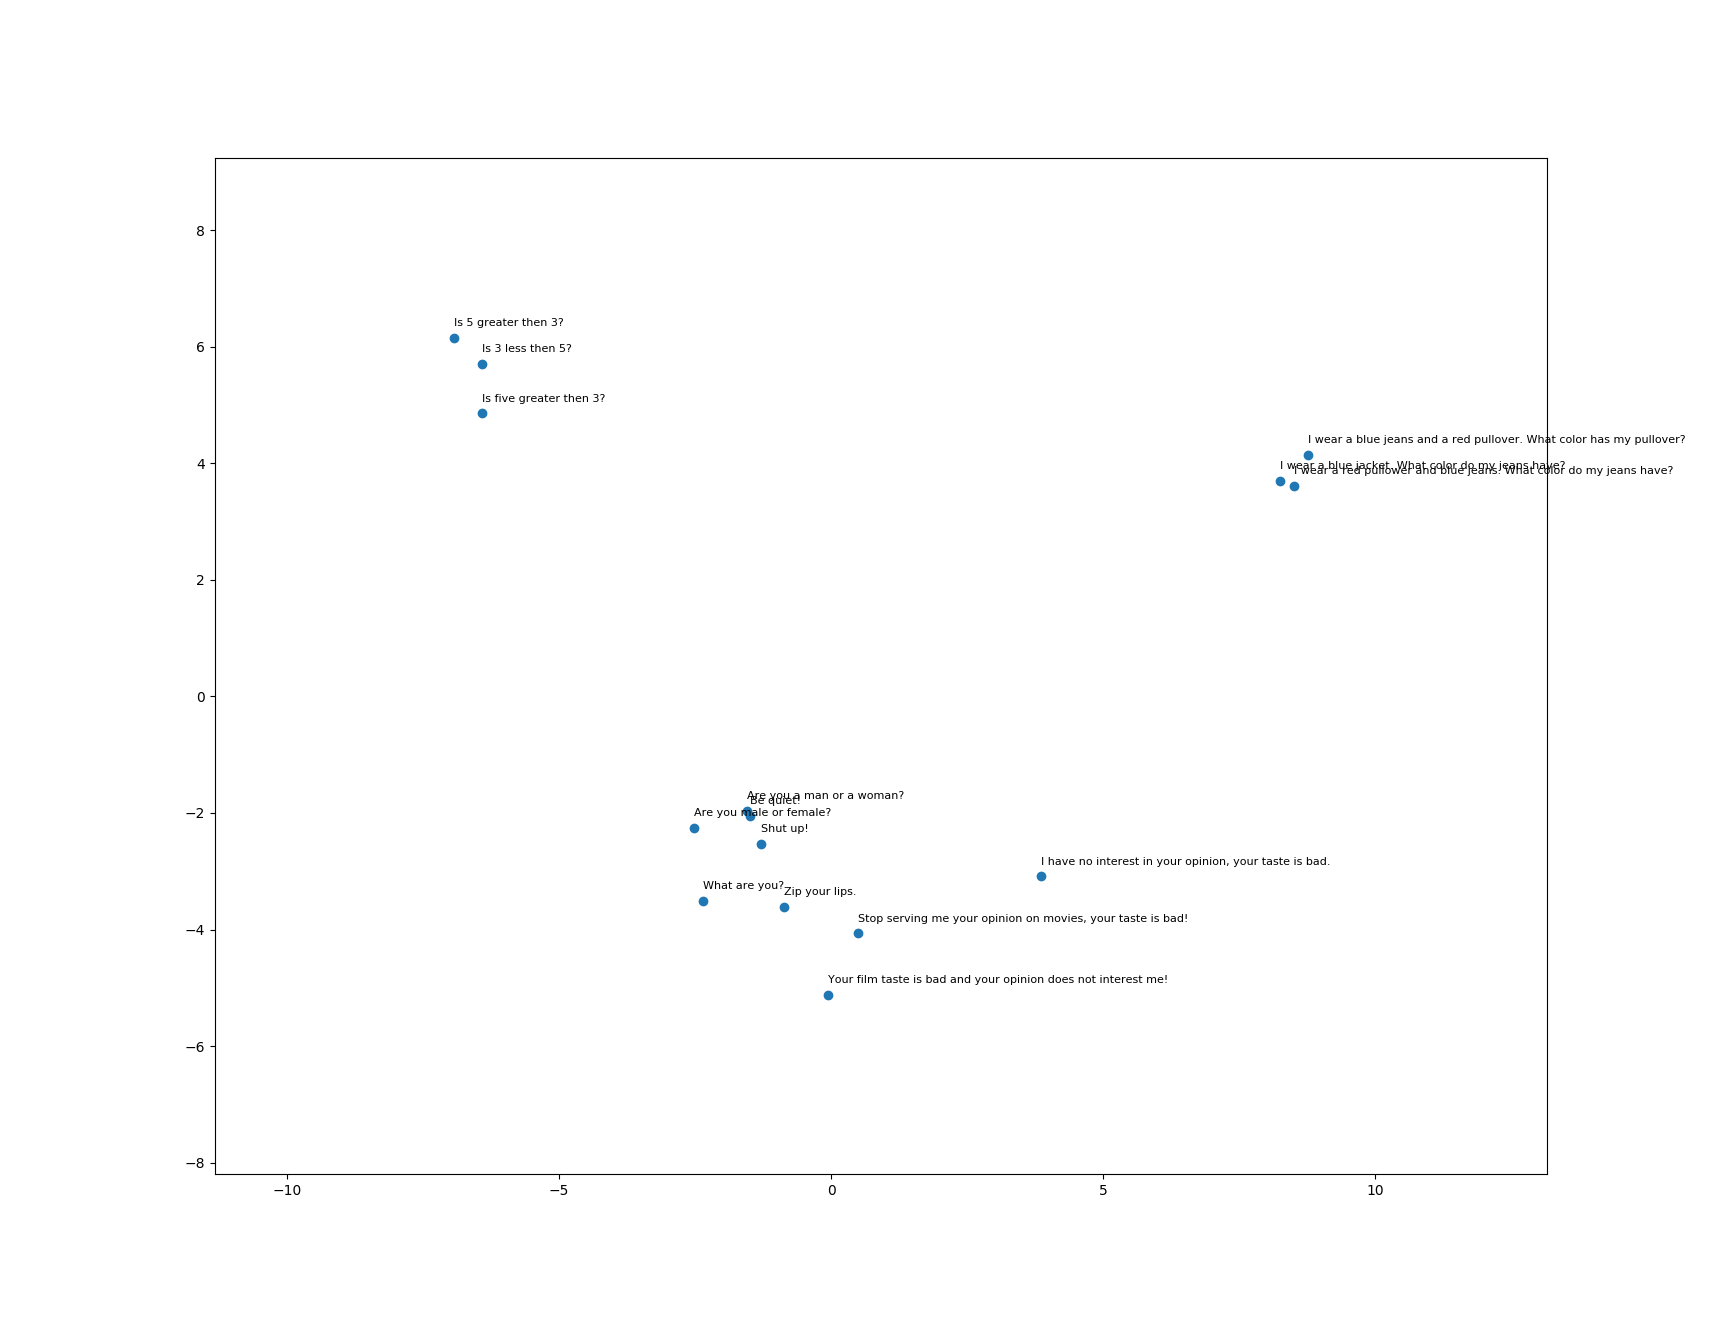
\includegraphics[width=16cm]{img/reddit_thought_vector_embeddings.png}
	\caption{The projected thought vectors for 15 different sentences when using the Reddit model. PCA was used for the projection.}
	\label{results:thougth_vectors:embeddings:reddit}
\end{figure}

Both of the models seem to have no problems understanding clear, direct sentences where the intent is clear (e.g. ``I have no interest in your opinion on movies, your taste is bad!''). This can be seen because similar sentences are clustered together in the projected space. However, when it comes to curses and questions regarding the gender, the OpenSubtitles model starts to struggle, which can be seen by taking a look at the respective points in the projected space. For example, the questions regarding the gender or the curses are scattered throughout the space, even though they should have been embedded closely to each other. The Reddit model seems to have less problems with this, as the embeddings for these sentences are quite close together. But what is interesting to see is that the Reddit model embeds the sentences with curses close to the sentences regarding the gender.\todo{write more}

\subsection{Attention??}\todo{move to own chapter at the end} 
\todo{noch entscheiden, ob wir das kapitel wollen}

\section{Comparison with Other Models}
As the next part, we want to compare the results of our model with two others we use as a reference: The CleverBot\footnote{http://www.cleverbot.com/} chatbot and the results from the paper ``Neural Conversational Model''~\cite{Vinyals:2015}, whose model architecture serves as the base of our model.\todo{name differences?} We test the quality of the responses from our models when confronted with utterances of different type and difficulty. We do this in the hope that we can reveal where the strengths and weaknesses of our models lie.

\subsection{Cleverbot}
\label{results:comparison:cleverbot}
We start with the comparison with the CleverBot. Keep in mind, that the CleverBot is a non-deterministic chatbot which means that the responses might be different if it is fed with the same inputs but a different point in time. The responses listed below were generated at the first of June between 12am and 15am.

\paragraph{Simple Utterance} We start by using the two simple utterances ``How are you?'' and ``Hi there, i m john!''. As one can see in the Tables~\ref{results:example1_output:OpenSubtitle_compared} and~\ref{results:example1_output:Reddit_compared}, both our OpenSubtitles model and the CleverBot answered this question with satisfying responses. The responses of the Reddit model to the utterance ``Hi there, i m john!'' are pretty bad as none of them is really useful. The response of the CleverBot to this utterance makes more sense in this case.
\\
\begin{table}[H]
	\centering
	\ra{1.3}
	\begin{adjustbox}{max width=\textwidth}
		\begin{tabular}{ll}
			\toprule
			Input: 	& \texttt{Hi, how are you?}\\
			\midrule
			0.5M: 	& \texttt{how are you ?}\\
			1.0M: 	& \texttt{i m fine}\\
			1.5M:	& \texttt{i m good}\\
			2.0M:	& \texttt{good}\\
			2.5M:	& \texttt{good}\\
			3.0M:	& \texttt{good}\\
			Cleverbot:	& \texttt{I'm good. How are you?}\\
			\bottomrule
		\end{tabular}
	\end{adjustbox}
\caption{Responses from the OpenSubtitles model for each snapshot, compared to the CleverBot response. The input utterance is ``How are you?''.}
\label{results:example1_output:OpenSubtitle_compared}

\end{table}
\begin{table}[H]
	\centering
	\ra{1.3}
	\begin{adjustbox}{max width=\textwidth}
		\begin{tabular}{ll}
			\toprule
			Input: 	& \texttt{Hi there, i m john!}\\
			\midrule
			0.5M:	& \texttt{<unknown>}\\
			1.0M: 	& \texttt{i m not a fan of the <unknown> , but i m not sure if you re a <unknown> .}\\
			1.5M: 	& \texttt{i m not the only one who thought this was a good idea .}\\
			2.0M:	& \texttt{i m a <unknown> !}\\
			2.5M:	& \texttt{i m not your buddy , guy .}\\
			3.0M:	& \texttt{i m not .}\\
			Cleverbot:	& \texttt{So what are you doing?}\\
			\bottomrule
		\end{tabular}
	\end{adjustbox}
	\caption{sponses from the Reddit model for each snapshot, compared to the CleverBot response. The input utterance is ``Hi there, i m john!''.}
	\label{results:example1_output:Reddit_compared}
\end{table}

\paragraph{Closed Question} As next, we are trying to see which responses are produced when using a closed question as the utterance. The results can be seen in the Tables~\ref{results:example2_output:OpenSubtitle_compared} and~\ref{results:example2_output:Reddit_compared}. With this type of utterance, we would like to evaluate if the models understand a closed question and can respond appropriately.

From the looks it seems that our models can respond to closed questions appropriately, as both of them gave appropriate answers. The CleverBot has problems with this question, probably because it does not understand how the concepts of flying and birds are related.
\\
\begin{table}[H]
	\centering
	\ra{1.3}
	\begin{adjustbox}{max width=\textwidth}
		\begin{tabular}{ll}
			\toprule
			Input: 	& \texttt{Can birds fly?}\\
			\midrule
			0.5M: 	& \texttt{no}\\
			1.0M: 	& \texttt{i can t}\\
			1.5M:	& \texttt{yeah , but in the meantime , i can t swim}\\
			2.0M:	& \texttt{no}\\
			2.5M:	& \texttt{i can t}\\
			3.0M:	& \texttt{sure}\\
			Cleverbot:	& \texttt{Some say they can.}\\
			\bottomrule
		\end{tabular}
	\end{adjustbox}
	\caption{Responses to a contextual question from the OpenSubtitles models and the CleverBot response.}
	\label{results:example2_output:OpenSubtitle_compared}
\end{table}
\begin{table}[H]
	\centering
	\ra{1.3}
	\begin{adjustbox}{max width=\textwidth}
		\begin{tabular}{ll}
			\toprule
			Input: 	& \texttt{Can birds fly?}\\
			\midrule
			0.5M: 	& \texttt{i m not sure if this is a movie , but i m not sure if it s a movie .}\\
			1.0M: 	& \texttt{i can not imagine how much i can get this .}\\
			1.5M:	& \texttt{i m sure he s a <unknown> .}\\
			2.0M:	& \texttt{yes}\\
			2.5M:	& \texttt{yes}\\
			3.0M:	& \texttt{yes}\\
			Cleverbot:	& \texttt{Some of them can.}\\
			\bottomrule
		\end{tabular}
	\end{adjustbox}
	\caption{Responses to a closed question from the Reddit models and the CleverBot response.}
	\label{results:example2_output:Reddit_compared}
\end{table}

\paragraph{Knowledge Question}
The next kind of utterance are knowledge questions. With this kind of questions we would like to evaluate if the models have knowledge about the world. The results can be seen in the Tables~\ref{results:example3_output:OpenSubtitle_compared} and~\ref{results:example3_output:Reddit_compared}.

The responses to the question about the color of the sky have an interesting development. Until the snapshot 2.0M, the responses were not appropriate and did not have any meaningful content\footnote{The response ``the jews'' comes from the fact, that in the beginning of the OpenSubtitles dataset, there are a lot of conversations related to movies about Nazism.}. However, from the snapshot 2.0M on the model answered in a correct way, even though it one time replied with red as the answer, which is obviously wrong. But it also had it right two times, whereas the last response from the 3.0M seems to be the best. The answer of the CleverBot to this question is quite meaningless and has absolutely nothing to do with the provided question.

The response to the question where the Reddit model lives was answered in a satisfying way, maybe except for the response of the 2.0M snapshot. It clearly understands the context of the question, as it always answers with a location-related answer. The CleverBot answers this question completely correct.

\begin{table}[H]
	\centering
	\ra{1.3}
	\begin{adjustbox}{max width=\textwidth}
		\begin{tabular}{ll}
			\toprule
			Input: 	& \texttt{What color is the sky?}\\
			\midrule
			0.5M: 	& \texttt{the jews}\\
			1.0M: 	& \texttt{it s a}\\
			1.5M:	& \texttt{oh , it s not}\\
			2.0M:	& \texttt{it s the blue}\\
			2.5M:	& \texttt{the red}\\
			3.0M:	& \texttt{blue}\\
			Cleverbot:&\texttt{*Kisses playfully*.}\\
			\bottomrule
		\end{tabular}
	\end{adjustbox}
	\caption{Responses to a knowledge question with the OpenSubtitles models and the CleverBot response.}
	\label{results:example3_output:OpenSubtitle_compared}
\end{table}
\begin{table}[H]
	\centering
	\ra{1.3}
	\begin{adjustbox}{max width=\textwidth}
		\begin{tabular}{ll}
			\toprule
			Input: 	& \texttt{In which country do you live?}\\
			\midrule
			0.5M: 	& \texttt{i m not sure if you re a <unknown> .}\\
			1.0M: 	& \texttt{i live in canada .}\\
			1.5M:	& \texttt{i live in the uk .}\\
			2.0M:	& \texttt{the country}\\
			2.5M:	& \texttt{canada}\\
			3.0M:	& \texttt{sweden}\\
			Cleverbot:&\texttt{The United States.}\\
			\bottomrule
		\end{tabular}
	\end{adjustbox}
	\caption{Responses to a knowledge question from the Reddit models and the CleverBot response.}
	\label{results:example3_output:Reddit_compared}
\end{table}

\paragraph{Contextual Question} 
With the next question, we want to try to evaluate if the models are capable of using contextual informations to build an appropriate response. The results can be seen in the Tables~\ref{results:example4_output:OpenSubtitle_compared} and~\ref{results:example4_output:Reddit_compared}.

As visible below, the OpenSubtitles models has big problems with this kind of utterances, as all the responses are not fitting. The only response that is close to being useful is the one of the 2.5M model, where it at least includes the right color in the response. The response of the CleverBot is in this case also not of relevance.

The responses of the Reddit model are more fitting to the question, but they are also pretty bad in comparison to what we have expected. At least it tries to formulate responses where the two colors of the question are comprised. The answer of the CleverBot is again useless, this time even more in comparison with the response given when using the question from the OpenSubtitles model.
\\
\begin{table}[H]
	\centering
	\ra{1.3}
	\begin{adjustbox}{max width=\textwidth}
		\begin{tabular}{ll}
			\toprule
			Input: 	& \texttt{I wear a blue jeans. What color do my jeans have?}\\
			\midrule
			0.5M: 	& \texttt{<unknown> <unknown>}\\
			1.0M: 	& \texttt{i don t know}\\
			1.5M:	& \texttt{oh , yeah}\\
			2.0M:	& \texttt{i m not a prostitute}\\
			2.5M:	& \texttt{i got a blue blue}\\
			3.0M:	& \texttt{i m not a fan}\\
			Cleverbot:	& \texttt{You don't have any.}\\
			\bottomrule
		\end{tabular}
	\end{adjustbox}
	\caption{Responses to a contextual question from the OpenSubtitles models and the CleverBot response.}
	\label{results:example4_output:OpenSubtitle_compared}
\end{table}
\begin{table}[H]
	\centering
	\ra{1.3}
	\begin{adjustbox}{max width=\textwidth}
		\begin{tabular}{ll}
			\toprule
			Input: 	& \texttt{I wear a red pullover and blue jeans. What color do my jeans have?}\\
			\midrule
			0.5M: 	& \texttt{i m a big fan of the <unknown> .}\\
			1.0M: 	& \texttt{i m not a fan of the <unknown> , but i do nt know what you re talking about .}\\
			1.5M:	& \texttt{i m a white male and i wear pants .}\\
			2.0M:	& \texttt{i wear a red shirt and i wear glasses .}\\
			2.5M:	& \texttt{i m a red blue and blue blue .}\\
			3.0M:	& \texttt{i m a white male and i have a blue blue shirt .}\\
			Cleverbot:	& \texttt{What is your opinion on President Obama. And don't ask me mine without saying}\\
			& \texttt{yours first!.}\\
			\bottomrule
		\end{tabular}
	\end{adjustbox}
	\caption{Responses to a contextual question from the Reddit models and the CleverBot response.}
	\label{results:example4_output:Reddit_compared}
\end{table}

\paragraph{Specific Question}
The next questions are more specific, we are going to ask the OpenSubtitles model a simple mathematical question and the Reddit models a question about the TV series ``Game of Thrones''. The results can be seen in the Tables~\ref{results:example5_output:OpenSubtitle_compared} and~\ref{results:example5_output:Reddit_compared}.

The responses of the OpenSubtitles in the beginning are quite clear, it does not know the answer or does not understand the question at all. However, the later snapshots (i.e. from 2.0M on), it seems to understand that it has to answer with a number. Sadly, the correct results is not in the generated responses. The CleverBot also does not understand how to answer such a question.

The Reddit model has an interesting twist in its responses. In the beginning, it starts by responding with generic responses which do not seem to have anything to do with the series itself. However, the funny response\footnote{``Hodor'' is a character in the ``Game of Thrones'' series who is only capable of saying its own name. In case of danger he starts yelling its name over and over several time throughout the series.} at the end indicates that it understands the question at least to some degree, even though the response does not contain any actual information about the series. The CleverBot response is a mysterious to us, as we cannot remember any scene from the series where a ``Dani'' plays a major role.
\\
\begin{table}[H]
	\centering
	\ra{1.3}
	\begin{adjustbox}{max width=\textwidth}
		\begin{tabular}{ll}
			\toprule
			Input: 	& \texttt{How much is 1 added to 2?}\\
			\midrule
			0.5M: 	& \texttt{i don t know}\\
			1.0M: 	& \texttt{i don t know}\\
			1.5M:	& \texttt{i don t know}\\
			2.0M:	& \texttt{ten dollars}\\
			2.5M:	& \texttt{50}\\
			3.0M:	& \texttt{2}\\
			Cleverbot:	& \texttt{I don't know.}\\
			\bottomrule
		\end{tabular}
	\end{adjustbox}
	\caption{Responses to a mathematical question from the OpenSubtitles models and the CleverBot response.}
	\label{results:example5_output:OpenSubtitle_compared}
\end{table}
\begin{table}[H]
	\centering
	\ra{1.3}
	\begin{adjustbox}{max width=\textwidth}
		\begin{tabular}{ll}
			\toprule
			Input: 	& \texttt{Can you tell me something about game of thrones?}\\
			\midrule
			0.5M: 	& \texttt{i m not sure if you re a fan of the movie , but i m not sure if you re going to be}\\
			& \texttt{a fan of the}\\
			1.0M: 	& \texttt{i m not sure what you re saying .}\\
			1.5M:	& \texttt{i m not sure if i m going to be watching this .}\\
			2.0M:	& \texttt{i m not sure if you re joking , but i m pretty sure that s the case .}\\
			2.5M:	& \texttt{i m not sure if you re talking about the game or the game , but i think the game}\\
			& \texttt{is a little different .}\\
			3.0M:	& \texttt{hodor hodor hodor hodor hodor hodor hodor hodor hodor hodor hodor hodor hodor hodor }\\
			& \texttt{hodor hodor hodor hodor hodor hodor hodor hodor hodor hodor hodor hodor hodor hodor}\\
			Cleverbot:	& \texttt{Dani is life.}\\
			\bottomrule
		\end{tabular}
	\end{adjustbox}
	\caption{Responses to a question about a TV series from the Reddit models and the CleverBot response.}
	\label{results:example5_output:Reddit_compared}
\end{table}

\paragraph{Answers to Statements}
Until now, we have only asked questions to our models. We would now like to see how the responses are if we input a statement instead of a question. The results can be seen in the Tables~\ref{results:example6_output:OpenSubtitle_compared} and~\ref{results:example6_output:Reddit_compared}.

The responses of the OpenSubtitles model are useful from the snapshot 2.0M and forward. Especially the answer for the snapshot 2.0M is interesting, as this seems to indicate that the model has some kind of empathy for the other person in the dialog, as it say ``i m sorry''. The response of the CleverBot signifies that it understands the statement to some degree, but does not know what to answer.

The responses of the Reddit model to the statement that it has a bad opinion are pretty bad across the board, with the response from the 1.5M model being the only one which is useful. The response of the CleverBot is a pretty speedy answer in this case.
\\
\begin{table}[H]
	\centering
	\ra{1.3}
	\begin{adjustbox}{max width=\textwidth}
		\begin{tabular}{ll}
			\toprule
			Input: 	& \texttt{i invited her to a public reading of my work , but she never came .}\\
			\midrule
			0.5M: 	& \texttt{she was a}\\
			1.0M: 	& \texttt{i don t know}\\
			1.5M:	& \texttt{really ?}\\
			2.0M:	& \texttt{i m sorry}\\
			2.5M:	& \texttt{she s been in a lot of trouble}\\
			3.0M:	& \texttt{she s not a fan}\\
			Cleverbot:	& \texttt{Who?}\\
			\bottomrule
		\end{tabular}
	\end{adjustbox}
	\caption{Responses to a statement from the OpenSubtitles models and the CleverBot response.}
	\label{results:example6_output:OpenSubtitle_compared}
\end{table}
\begin{table}[H]
	\centering
	\ra{1.3}
	\begin{adjustbox}{max width=\textwidth}
		\begin{tabular}{ll}
			\toprule
			Input: 	& \texttt{Your film taste is bad and your opinion does not interest me!}\\
			0.5M: 	& \texttt{i m not sure what you re saying .}\\
			1.0M: 	& \texttt{i m not your friend , but i m not a fan of the <unknown> .}\\
			1.5M:	& \texttt{i m sorry , i did nt know that .}\\
			2.0M:	& \texttt{i m not a fan of the movie , but i m not sure if you re going to be a fan of the film .}\\
			2.5M:	& \texttt{i m not a fan of the film , but i think it s a good movie .}\\
			3.0M:	& \texttt{i m not sure if you re being sarcastic or not .}\\
			Cleverbot:	& \texttt{And for me your opinion does not matter.}\\
			\bottomrule
		\end{tabular}
	\end{adjustbox}
	\caption{Responses to a statement from the Reddit models and the CleverBot response.}
	\label{results:example6_output:Reddit_compared}
\end{table}

\paragraph{Self-Concept} At the end, we have an interesting answer from the Reddit model to the question ``What are you?''. The responses can be seen in Table~\ref{results:example7_output:Reddit_compared}. All snapshots produce bad responses, apart from the last, which answered that it is a bot. This is an interesting answer because it shows that the model seems to have some kind of self-concept. We cannot explain that, as the model was trained on comments from Reddit discussion about movies and series. Nevertheless, it is an interesting answer to see.

\begin{table}[H]
	\centering
	\ra{1.3}
	\begin{adjustbox}{max width=\textwidth}
		\begin{tabular}{ll}
			\toprule
			Input: 	& \texttt{What are you?}\\
			0.5M: 	& \texttt{i m not a fan of the movie , but i m a huge fan of the movie .}\\
			1.0M: 	& \texttt{i m not a fan of the <unknown> , but i m not a fan of the <unknown> .}\\
			1.5M:	& \texttt{i m not .}\\
			2.0M:	& \texttt{i m not .}\\
			2.5M:	& \texttt{i m not .}\\
			3.0M:	& \texttt{i m a bot .}\\
			Cleverbot:	& \texttt{A human, what are you??}\\
			\bottomrule
		\end{tabular}
	\end{adjustbox}
	\caption{Responses to a self-concept question from the Reddit models and the CleverBot response..}
	\label{results:example7_output:Reddit_compared}
\end{table}

Sadly, we were not able to find a similar response when using the OpenSubtitles model.

\paragraph{Fazit}\todo{Fazit!}

\subsection{Neural Conversational Model}
\label{results:comparison:ncm}
In this section, we are going to compare the results from the paper ``Neural Conversation Model'' (NCM) with the results from our models. To compare the responses, we are going to use utterances from the paper and show all the responses from all OpenSubtitles snapshots, but only the (subjectively) best response from the Reddit model, as the NCM model was trained on the OpenSubtitles dataset. The responses can be seen in the Tables~\ref{results:example8_output:Neural_Conversational_Model_compared} to~\ref{results:example14_output:Neural_Conversational_Model_compared}. The categories where the input utterances came from in the paper are noted in the table descriptions.

We are only showing a part of the dialogs which were evaluated. All others can be found in Appendix~\ref{apendix:results:compared_with_NCM}.
\\
\begin{table}[H]
	\centering
	\ra{1.3}
	\begin{adjustbox}{max width=\textwidth}
		\begin{tabular}{ll}
			\toprule
			Input: 	& \texttt{what year were you born ?}\\
			\midrule
			OpenSubtitle\\
			0.5M: 	& \texttt{a lot of people}\\
			1.0M: 	& \texttt{i was a}\\
			1.5M:	& \texttt{a little}\\
			2.0M:	& \texttt{i was born}\\
			2.5M:	& \texttt{i don t know}\\
			3.0M:	& \texttt{i don t know}\\
			\midrule
			Reddit\\
			2.0M:	& \texttt{i was born in the 90s .}\\
			\midrule
			NCM:	& \texttt{1977 .}\\
			\bottomrule
		\end{tabular}
	\end{adjustbox}
	\caption{Comparison between the NCM model and our OpenSubtitles model when using a question from the ``Basic'' category in the paper.}
	\label{results:example8_output:Neural_Conversational_Model_compared}
\end{table}

\begin{table}[H]
	\centering
	\ra{1.3}
	\begin{adjustbox}{max width=\textwidth}
		\begin{tabular}{ll}
			\toprule
			Input: 	& \texttt{why are we here ?}\\
			\midrule
			OpenSubtitle\\
			0.5M: 	& \texttt{because we were here}\\
			1.0M: 	& \texttt{i don t know}\\
			1.5M:	& \texttt{i don t know}\\
			2.0M:	& \texttt{i m sorry}\\
			2.5M:	& \texttt{we re here}\\
			3.0M:	& \texttt{we re here}\\
			\midrule
			Reddit\\
			2.5M:	& \texttt{because we re here .}\\
			\midrule
			NCM:	& \texttt{i ’m not sure .}\\
			\bottomrule
		\end{tabular}
	\end{adjustbox}
	\caption{Comparison between the NCM model and our OpenSubtitles model when using a question from the ``Basic'' category in the paper.}
	\label{results:example9_output:Neural_Conversational_Model_compared}
\end{table}
\begin{table}[H]
	\centering
	\ra{1.3}
	\begin{adjustbox}{max width=\textwidth}
		\begin{tabular}{ll}
			\toprule
			Input: 	& \texttt{are you a leader or a follower ?}\\
			\midrule
			OpenSubtitle\\
			0.5M: 	& \texttt{no}\\
			1.0M: 	& \texttt{i m not a}\\
			1.5M:	& \texttt{i m sorry}\\
			2.0M:	& \texttt{i m not a prostitute}\\
			2.5M:	& \texttt{i m a}\\
			3.0M:	& \texttt{i m a}\\
			\midrule
			Reddit\\
			2.0M:	& \texttt{i m a cyborg .}\\
			\midrule
			NCM:	& \texttt{i'm a leader .}\\
			\bottomrule
		\end{tabular}
	\end{adjustbox}
	\caption{Comparison between the NCM model and our OpenSubtitles model when using a question from the ``General Knowledge Q\&A'' category in the paper.}
	\label{results:example10_output:Neural_Conversational_Model_compared}
\end{table}
\begin{table}[H]
	\centering
	\ra{1.3}
	\begin{adjustbox}{max width=\textwidth}
		\begin{tabular}{ll}
			\toprule
			Input: 	& \texttt{how much is ten minus two ?}\\
			\midrule
			OpenSubtitle\\
			0.5M: 	& \texttt{four}\\
			1.0M: 	& \texttt{ten}\\
			1.5M:	& \texttt{two , two , three}\\
			2.0M:	& \texttt{ten dollars}\\
			2.5M:	& \texttt{ten}\\
			3.0M:	& \texttt{ten}\\
			\midrule
			Reddit\\
			2.5M:	& \texttt{i m not sure what you re talking about .}\\
			\midrule
			NCM:	& \texttt{seventy - two .}\\
			\bottomrule
		\end{tabular}
	\end{adjustbox}
	\caption{Comparison between the NCM model and our OpenSubtitles model when using a question from the ``General Knowledge Q\&A'' category in the paper.}
	\label{results:example11_output:Neural_Conversational_Model_compared}
\end{table}
\begin{table}[H]
	\centering
	\ra{1.3}
	\begin{adjustbox}{max width=\textwidth}
		\begin{tabular}{ll}
			\toprule
			Input: 	& \texttt{what is the color of a yellow car ?}\\
			\midrule
			OpenSubtitle\\
			0.5M: 	& \texttt{a <unknown> ?}\\
			1.0M: 	& \texttt{it s a}\\
			1.5M:	& \texttt{what ?}\\
			2.0M:	& \texttt{it s a blue blue}\\
			2.5M:	& \texttt{it s a blue}\\
			3.0M:	& \texttt{it s a yellow}\\
			\midrule
			Reddit\\
			2.5M:	& \texttt{the yellow yellow yellow yellow yellow yellow yellow yellow}\\
					& \texttt{yellow yellow yellow yellow yellow yellow yellow yellow yellow}\\
					& \texttt{yellow yellow yellow yellow yellow yellow yellow yellow yellow yellow}\\
					\midrule
			NCM:	& \texttt{yellow .}\\
			\bottomrule
		\end{tabular}
	\end{adjustbox}
	\caption{Comparison between the NCM model and our OpenSubtitles model when using a question from the ``General Knowledge Q\&A'' category in the paper.}
	\label{results:example12_output:Neural_Conversational_Model_compared}
\end{table}
\begin{table}[H]
	\centering
	\ra{1.3}
	\begin{adjustbox}{max width=\textwidth}
		\begin{tabular}{ll}
			\toprule
			Input: 	& \texttt{what is the purpose of existence ?}\\
			\midrule
			OpenSubtitle\\
			0.5M: 	& \texttt{the jews}\\
			1.0M: 	& \texttt{i don t know}\\
			1.5M:	& \texttt{you re just a fucking boy , man}\\
			2.0M:	& \texttt{i don t know}\\
			2.5M:	& \texttt{i m sorry}\\
			3.0M:	& \texttt{i m not sure}\\
			\midrule
			Reddit\\
			1.5M:	& \texttt{i m not sure if you re joking or not , but i m sure you re }\\
			& \texttt{not familiar with the word .}\\
			\midrule
			NCM:	& \texttt{to find out what happens when we get to the planet earth .}\\
			\bottomrule
		\end{tabular}
	\end{adjustbox}
	\caption{Comparison between the NCM model and our OpenSubtitles model when using a question from the ``Philosophical Q\&A'' category in the paper.}
	\label{results:example13_output:Neural_Conversational_Model_compared}
\end{table}
\begin{table}[H]
	\centering
	\ra{1.3}
	\begin{adjustbox}{max width=\textwidth}
		\begin{tabular}{ll}
			\toprule
			Input: 	& \texttt{what are the things that i do to be immoral?}\\
			\midrule
			OpenSubtitle\\
			0.5M: 	& \texttt{i don t know}\\
			1.0M: 	& \texttt{i don t know}\\
			1.5M:	& \texttt{what s the big idea ?}\\
			2.0M:	& \texttt{i don t know}\\
			2.5M:	& \texttt{i m a}\\
			3.0M:	& \texttt{i m not a criminal}\\
			\midrule
			Reddit\\
			2.5M:	& \texttt{i think you re missing the point .}\\
			& \texttt{i don ’t know .}\\
			\midrule
			NCM:	& \texttt{to find out what happens when we get to the planet earth .}\\
			\bottomrule
		\end{tabular}
	\end{adjustbox}
	\caption{Comparison between the NCM model and our OpenSubtitles model when using a question from the ``Morality'' category in the paper.}
	\label{results:example14_output:Neural_Conversational_Model_compared}
\end{table}

\paragraph{Fazit} Es scheint so, dass unsere Modelle für einfachere Fragen gut funktionieren, für komplexere Fragen aber die Sprachvielfalt fehlt. \todo{vielleicht noch ergännzen, indem resultate pro Conversation genauer beschrieben werden. Zusätzlich vielleicht noch cpations überarbeiten}

\paragraph{Brings Beam-search Surprises?}\todo{Wenn wir die gleiche Struktur wie "immer" machen, müssten wir hier das Fazit des Vergleichs machen und dann mit einem Satz eine Überleitung zu Beam Search?}

\section{Beam-search}
There are always some bad replies in the examples seen above. To fix this, we would like to use a simple beam-search implementation as described in Chapter~\ref{fundamentals:decoding_approaches} to see if that helps to fix this problem. We will evaluate this for three different examples, and judge in a subjective if the responses generated by the beam-search decoder are superior to the responses of the greedy decoder. This is only done with the OpenSubtitle 3.0M snapshot and a beam-width of $200$.

\paragraph{``what year were you born?''} The responses of the greedy decoder to this question can be found in Chapter~\ref{results:comparison:ncm} in the Table~\ref{results:example8_output:Neural_Conversational_Model_compared}. The original answers of the OpenSubtitles model were all pretty bad, and it seemed that it did not fully understand the question.

However, when using the beam-search decoder, there are several useful responses, such as ``1991'', ``last year'' or ``five years ago''. This responses are much better than what the greedy decoder initially produced. However, they are not the highest ranked response and hence are not returned by the model if we only take a look at the best response.

\paragraph{``i wear a blue jeans. what color do my jeans have?''} \blindtext
\paragraph{``what is the purpose of being intelligent?''} \blindtext

\paragraph{Als Zweites} prüften wir die Responses der Input Utterance "I wear a blue jeans. What color do my jeans have?". Die Greedy decoding Resultate befinden sich hierzu im Kapitel \ref{?} in der Tabelle \ref{results:example4_output:OpenSubtitle_compared} und sind teilweise schlecht. Das 2.5M Modell liefert das beste Resultate mit "i got a blue blue", welches die erwünschte Antwort immerhin enhält. Der response des 3.0M war "i m not a fan", was für uns eine Kontextfreie utterance ist.\\

Die Antworten des Beam-search befinden sich im Anhang \ref{apendix:result2:Beam-search-200:OpenSubtitle}. Daruntern befinden sich gute Responses wie: "blue", "you know that". Wir sehen also auch hier 2 deutlich bessere responses als "i m not a fan".

\paragraph{Als Drittes} testen möchten wir die etwas schwierigere Aussage "what is the purpose of being intelligent?" mit Beam-search testen.
Die Antworten mit Greedy decoding befinden sich hier unterhalb in der Tabelle \ref{results:example20_output:OpenSubtitle} und bestehen fast ausschliesslich aus der generischen response "i don t know", welche zwar im Kontext korrekt ist, jedoch ist diese reponse für viele Fragen eine gute Antwort. 
Wir möchten herausfinden, ob mit Beam-search bessere und spannendere responses möglich sind.\\

Alle responses befinden sich im Anhang \ref{apendix:result3:Beam-search-200:OpenSubtitle}. Hier können nun mehrere Antworten als passend angesehen, da es eben eine philosophical question is. Hier ein einige gute Antworten:  "well , it s complicated", "you know ?", "you can t know", "well , it s nothing".

\begin{table}[H]
	\centering
	\ra{1.3}
	\begin{adjustbox}{max width=\textwidth}
		\begin{tabular}{ll}
			\toprule
			Input: 	& \texttt{what is the purpose of being intelligent?}\\
			\midrule
			OpenSubtitle\\
			0.5M: 	& \texttt{the jews}\\
			1.0M: 	& \texttt{i don t know}\\
			1.5M:	& \texttt{i don t know}\\
			2.0M:	& \texttt{i don t know}\\
			2.5M:	& \texttt{i don t know}\\
			3.0M:	& \texttt{i don t know}\\
			\midrule
			NCM:	& \texttt{to find out what it is .}\\
			\bottomrule
		\end{tabular}
	\end{adjustbox}
	\caption{Beispiel Vergleich aus Paper Neural Conversational Model Resultate Conversation 4: Philosophical Q\&A}
	\label{results:example20_output:OpenSubtitle}
\end{table}

\paragraph{Zusammenfassend} waren die Beam-search Resultate erfolgreich. Es ist jedoch schwierig, wie das beste Resultat ausgewählt werden soll. Dazu müsste man vermutlich wenn ein Modell trainieren, welches aus einem set von 200 replies den passendsten zu einem gegebene Input suchen. Vielleicht könnte man so eine bessere Qualität der Sprache erzielen. Aber wir können unmöglich über mehrere Checkpoints pro utterance jweils 200 responses auswerten. Deshalb konnten wir Beam-Search nicht für die Evaluierung der Modelle brauchen. Auch haben wir Beam-search nicht genau gemäss Theorie implementiert/nicht damit trainiert (hier weisst du vermutlich besser was schreiben, wenn wir das erwähnen möchten)
\section{Reverse Input Feeding}\todo{raus?}
\blindtext